	\documentclass[10pt,oneside]{CBFT_book}
	% Algunos paquetes
	\usepackage{amssymb}
	\usepackage{amsmath}
	\usepackage{graphicx}
	\usepackage{libertine}
% 	\usepackage[bold-style=TeX]{unicode-math}
	\usepackage{lipsum}

	\usepackage{natbib}
	\setcitestyle{square}

	\usepackage{polyglossia}
	\setdefaultlanguage{spanish}


	\usepackage{CBFT.estilo} % Cargo la hoja de estilo

	% Tipografías
	% \setromanfont[Mapping=tex-text]{Linux Libertine O}
	% \setsansfont[Mapping=tex-text]{DejaVu Sans}
	% \setmonofont[Mapping=tex-text]{DejaVu Sans Mono}

	%===================================================================
	%	DOCUMENTO PROPIAMENTE DICHO
	%===================================================================

% \title{CBFT Mecánica clásica}
% \author{Cuerpos rígidos}
% \date{\today}

\begin{document}
% \maketitle
% \tableofcontents
\chapter{Cuerpos rígidos}

% =================================================================================================
\section{Cuerpos rígidos}\index{Cuerpo rígido}
% =================================================================================================

Se pueden pensar como un sistema que interactúa a través de fuerzas de vínculo que están asociadas
a la {\it condición de rigidez}. Los vínculos constituyen la condición de rigidez,
\be
	|\vb{x}_i - \vb{x}_j | = d_{ij}	\qquad i \neq j
\label{vinculos}
\ee

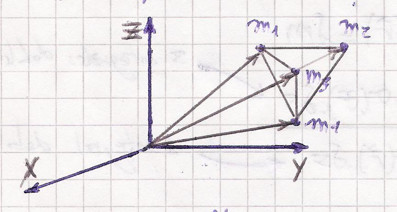
\includegraphics[scale=0.4]{images/fig_mc_rigid_body_1.jpg}

Se asocia entonces al conjunto discreto de partículas. Entonces 
\[
	T = \frac 1 2 \sum_i^N m_i v_i^2, 
\]
con la condición de rigidez de las $N$ partículas.

Luego se hace el pasaje del discreto al continuo, a través de la idea 
\[
	\delta m = \rho(\vb{x}) \delta V.
\]
Las partículas están tan próximas que se puede pensar en una distribución continua de masa 
donde la masa de cada partícula se transforma en la masa de $N$ {\it cubitos} pequeños, entonces 
\[
	\vb{R} = \frac{\sum_i m_i\vb{x}_i}{\sum_i m_i} \longrightarrow 
	\vb{R} = \frac{\int \rho \vb{x}_i dV }{\int \: \rho dV} 
\]

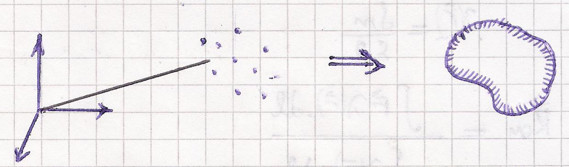
\includegraphics[scale=0.4]{images/fig_mc_rigid_body_2.jpg}

\notamargen{En relatividad restringida no existen cuerpos rígidos; a este nivel no nos preocupamos de ello.
Buscaremos escribir el lagrangiano de cada tipo de cuerpo.}

Se corta al cuerpo rígido en cubos (se particiona) y cada cubito se trata como las $m_i$ del caso discreto.

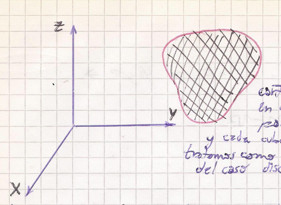
\includegraphics[scale=0.4]{images/fig_mc_rigid_body_3.jpg}

Como el volumen $V$ del cuerpo es constante, se tiene 
\[
	\lim_{N\to\infty,\delta V\to 0} \delta V N = V
\]
y el centro de masa cumple 
\[
	\vb{R} = \frac{\sum_i \vb{x}_i \rho(\vb{x}_i) \delta V }{\sum_i \rho(\vb{x}_i) \delta V}  \to 
	\frac{\int \rho(\vb{x}) \vb{x} dV }{\int \: \rho dV}, 
\]
donde debemos notar que el numerador tiene el carácter vectorial porque son tres integrales triples.

Otros cuerpos rígidos son los que tienen una o dos dimensiones despreciables (una lámina o un alambre, respectivamente)
que se pueden modelar considerando distribuciones de masa superficiales o longitudinales,
\[
	\sigma(\vb{x}) = \frac{\delta m}{\delta S}, \quad \lambda(\vb{x}) = \frac{\delta m}{\delta \ell}
\]

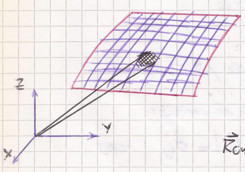
\includegraphics[scale=0.4]{images/fig_mc_rigid_body_4.jpg}

Para el caso 2D, será
\[
	\vb{R} = \frac{ \int_S \vb{x} \sigma{\vb{x}} dS }{ \int_S \sigma{\vb{x}} dS },
\]
y correspondientemente en el caso 1D
\[
	\vb{R} = \frac{ \int \vb{x} \lambda{\vb{x}} d\ell }{ \int \lambda{\vb{x}} d\ell }.
\]

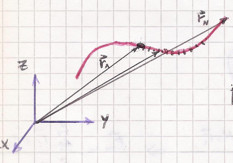
\includegraphics[scale=0.4]{images/fig_mc_rigid_body_5.jpg}

Obviamente las abreviaturas $\rho, \sigma, \lambda$ son una convención nuestra. Prestar atención a las unidades.

% ~~~~~~~~~~~~~~~~~~~~~~~~~~~~~~~~~~~~~~~~~~~~~~~~~~~~~~~~~~~~~~~~~~~~~~~~~~~~~~~~~~~~~~~~~~~~~~~~~~~~~~~~~~~~~~~
\subsection{Grados de libertad de un cuerpo rígido}\index{Cuerpo rígido, grados de libertad}

Consideremos un cuerpo rígido de 5 grados de libertad como el de la figura,

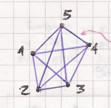
\includegraphics[scale=0.4]{images/fig_mc_rigid_body_6.jpg}

Vemos que de entrada son $(N 2)$ ecuaciones de vínculo (nro combinatorio) de manera que en este caso se tendrían
$ 3\times5 - 10 = 5 $ grados de libertad. Pero esto está mal; estas ecuaciones sucede que no son independientes.
\notamargen{Chequear lo del combinatorio y el resultado 10. No lo veo así fácil de una.}

Cada punto tiene como vínculos las ecuaciones \eqref{vinculos}

\begin{figure}[htb]
	\begin{center}
	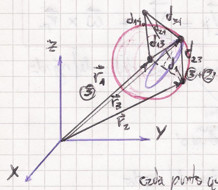
\includegraphics[width=0.6\textwidth]{images/fig_mc_rigidgl.pdf}	 
	\end{center}
	\caption{}
\end{figure} 

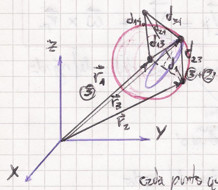
\includegraphics[scale=0.4]{images/fig_mc_rigidgl.jpg}

Examinando el dibujo de la figura sobre estas líneas vemos [¿?] que el segundo punto estará a distancia $d_1$ de
cualquier punto sobre la esfera (necesito dos coordenadas más). Para el punto 3 necesito un ángulo (una coordenada).
Al agregar los siguientes puntos no se requieren nuevas coordenadas; cada punto que agrego viene con la distancia a
todos los otros. Entonces, en tres dimensiones un cuerpo rígido tiene seis grados de libertad.

Si las condiciones de rigidez son lineales resultan cinco grados de libertad.

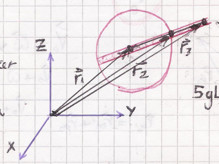
\includegraphics[scale=0.4]{images/fig_mc_rigid_body_7.jpg}

En un cuerpo lineal no tiene sentido la rotación del tercer punto $\vb{x}_3$, entonces ahi se {\it pierde} una
coordenada.


% ~~~~~~~~~~~~~~~~~~~~~~~~~~~~~~~~~~~~~~~~~~~~~~~~~~~~~~~~~~~~~~~~~~~~~~~~~~~~~~~~~~~~~~~~~~~~~~~~~~~~~~~~~~~~~~~
\subsection{Velocidad de un cuerpo rígido}\index{Cuerpo rígido, velocidad}

Lo único que pueden hacer los puntos de un cuerpo rígido, respecto de otro punto del mismo, es rotar puesto que
el módulo de la distancia debe permanecer constante.

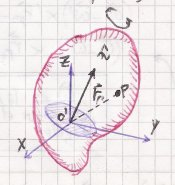
\includegraphics[scale=0.4]{images/fig_mc_rigid_body_vel1.jpg}

Con respecto a este gráfico superior, la construcción mostrada significa que 

\begin{figure}[htb]
	\begin{center}
	\includegraphics[width=0.35\textwidth]{images/fig_mc_rigidvel.pdf}	 
	\end{center}
	\caption{}
\end{figure} 

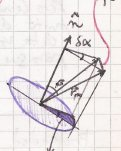
\includegraphics[scale=0.4]{images/fig_mc_rigid_body_vel2.jpg}

\[
	\delta r_{p_0} = r_{p_0} \sin(\beta) \delta \alpha = | \delta \vb{r}_{p_0} |
\]

Luego, el módulo de la velocidad es 
\[
	\lim_{\delta t \to 0} \frac{\delta r_{p_0}}{\delta t} = 
	r_{p_0} \sin(\beta) \frac{\delta\alpha}{\delta t},
\]
o bien 
\[
	v_{p_0} = \dot{\alpha} \: r_{p_0} \sin(\beta)
\]

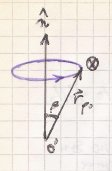
\includegraphics[scale=0.4]{images/fig_mc_rigid_body_vel3.jpg}

Dadas las direcciones mostradas en la figura de arriba se ve que la fórmula es el
módulo de un producto vectorial entre $\dot{\alpha} \equiv \omega$ y $\vb{r}_p$ y como el resultado
es perpendicular a $\vb{r}_p$ y al vector $\hat{n}$ se tiene $\vb{\omega} = \omega \hat{n}$.

pero $v_{p_0} \perp \hat{n}$ y $v_{p_0} \perp r_{p_0}$ de manera que 
\[
	\vb{v}_{p_0} = \vb{\Omega} \times \vb{r}_{p_0},
\]
es la velocidad de rotación.
Pero necesito ir a un sistema inercial para poder definir una velocidad que sirva para el
cálculo del lagrangiano.

Luego, para ir a un sistema inercial le sumo la V de algún punto del rígido (el origen O)
medido desde un sistema inercial. Entonces, el campo de velocidad del cuerpo rígido es
\[
	\vb{v}_{p} = \vb{v}_O + \vb{\Omega} \times \vb{r}_{p_0}.
\]
de manera que la velocidad en un punto $p$ es la suma entre el producto vectorial visto y 
la velocidad del orignen no inercial $O$.
\notamargen{La velocidad en el RHS es la medida desde un sistema inercial; tiene que quedar
claro eso!}


\subsection{Unicidad de la velocidad de rotación}

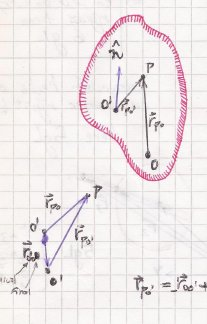
\includegraphics[scale=0.4]{images/fig_mc_rigid_body_vel4.jpg}

Desde dos puntos arbitrarios del rígido $0$ y $0'$, tomados como origen de un sistema no inercial
de coordenadas, se puede escribir la velocidad de otro punto $P$ como
\[
	\vb{V}_{p} = \vb{V}_0' + \vb{\Omega}' \times \vb{r}_{p_0'}
\]
siendo \vb{\Omega}' la \vb{\Omega} como se ve desde el sistema O'
\[
	\vb{V}_{p} = \vb{V}_0 + \vb{\Omega} \times \vb{r}_{p_0}
\]
y donde \vb{\Omega} es la vista desde el sistema O.
\begin{figure}[htb]
	\begin{center}
	\includegraphics[width=0.35\textwidth]{images/fig_mc_velrot.pdf}	 
	\end{center}
	\caption{}
\end{figure} 
\[
	\vb{V}_0' + \vb{\Omega}' \times \vb{r}_{p_0'} = \vb{V}_0 + \vb{\Omega} \times \vb{r}_{p_0} 
\]
y descomponiendo de acuerdo con el dibujo resulta 
\[
	\vb{\Omega} \times \vb{r}_{OO'} + \vb{\Omega}' \times \vb{r}_{0'p} = \vb{\Omega} \times \vb{r}_{p_0} 
\]
\[
	\vb{\Omega} \times ( \vb{r}_{00'} - \vb{r}_{0p} ) + \vb{\Omega}' \times \vb{r}_{0'p}  = 0
\]
\[
	( \vb{\Omega}' - \vb{\Omega}  ) \times \vb{r}_{0'p} = 0.
\]
Pero como $\vb{r}_{0'p}$ es cualquier punto del cuerpo rígido, debe darse que el paréntesis es nulo, de
lo cual se deduce que $\vb{\Omega}'=\vb{\Omega}$. Entonces, \vb{\Omega} es la misma para cualquier
punto del cuerpo rígido.

Notemos la siguiente propiedad que emerge del producto escalar;
\[
	\vb{\Omega} \cdot \vb{V}_p = \vb{\Omega} \cdot \vb{V}_0 +
	\vb{\Omega}\cdot(\vb{\Omega}\times \vb{r}_{0p} )
\]
\[
	\vb{\Omega} \cdot \vb{V}_p = \vb{\Omega} \cdot \vb{V}_0
\]
lo cual se cumple para todo punto $p$ perteneciente al cuerpo rigido. Si es $\vb{\Omega} \cdot \vb{V}_0 = 0$
entonces serán $\vb{\Omega} \perp \vb{V}_0$ y $\vb{\Omega} \perp \vb{V}_p$.

Si desde un sistema inercial vemos que $\vb{\Omega} \perp \vb{v}_p$ entonces para todos los puntos del 
cuerpo \vb{\Omega}  es perpendicular a cualquier punto.

Si en un instante dado \vb{\Omega} es perpendicular a $\vb{V}_p$ entonces \vb{\Omega} es perpendicular a 
$\vb{V}_{p'}$ para todo punto del cuerpo rígido.

Si en un instante dado un punto es perpendicular a $\vb{\omega}$ entonces todos los puntos lo son.
El cuerpo está sufriendo una rotación pura. Los puntos se mueven en una dirección o se mueven en la contraria.

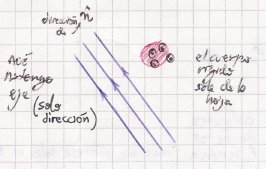
\includegraphics[scale=0.4]{images/fig_mc_rigid_body_vel5.jpg}

La propiedad que acabamos de analizar garantiza que hay una rotación en torno algún eje; otra
historia diferente es encontrarlo.

\subsection{Eje instantáneo de rotación}


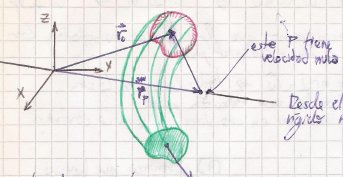
\includegraphics[scale=0.4]{images/fig_mc_rigid_body_ejerot.jpg}
 
Si $p$ es tal que $\vb{V}_p = 0$ entonces
\be
	\vb{V}_0 = - \vb{\Omega} \times \vb{r}_{p0}
	\label{condicion_eje}
\ee
donde $\vb{V}_0$ es una velocidad desde un sistema inercial.
Desde el sistema inercial el cuerpo rígido realiza una rotación pura, puesto que veo al
punto O rotar en torno a algún eje.
Es decir que el punto P determina un eje.
\[
	\vb{V}_0 = - \vb{\Omega} \times ( r_{\perp} + r_{\parallel} ) = -\vb{\Omega} \times  r_{\perp} 
\]
y esto define un eje instantáneo de rotación.

Como vale \eqref{condicion_eje} se da que cualquiera de los \vb{r} de la figurilla debajo

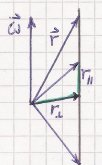
\includegraphics[scale=0.4]{images/fig_mc_rigid_body_ejerot2.jpg}

verifica la condición predicha. Solo interesa la parte perpendicular.
En este caso el cuerpo tiene un eje instantáneo de rotación.

\begin{figure}[htb]
	\begin{center}
	\includegraphics[width=0.3\textwidth]{images/fig_mc_ejeinst.pdf}	 
	\end{center}
	\caption{}
\end{figure} 

Se puede hallar un origen $O$ tal que verifique 
\[
	\vb{v}_p = \vb{v}_0^\perp + \vb{v}^\parallel + \vb{\omega} \times \vb{r}_{p_0}  
\]

El movimiento más general de un cuerpo rígido es de traslación y de rotación combinados.

% =================================================================================================
\section{Energía cinética del cuerpo rígido}
% =================================================================================================

\notamargen{Los vínculos del cuerpo rígido son holónomos, entonces podemos usar el lagrangiano $Lag$ [?]}
Queremos escribir la energía cinética de un cuerpo rígido explícitamente en términos del momento
de inercia $I$.
\[
	T = \frac{1}{2} \sum_i^N m_i v_i^2 = \frac{1}{2} \sum_i^N m_i ( \vb{v}_{cm} + \vb{\Omega} \times \vb{r}_i ) ^2
\]
donde la última $\vb{r}_i$ está referida al centro de masa (posiciones de los puntos del cuerpo
rígido referidas al centro de masa).
\[
	T = \frac{1}{2} \sum_i^N m_i ( \vb{v}_{cm}^2 + (\vb{\Omega} \times \vb{r}_i)^2 +
		2 \vb{v}_{cm} \cdot (\vb{\Omega} \times \vb{r}_i)  )
\]
pero es fácil ver que el término de cruza es cero dado que 
\[
	\sum_i^N m_i \vb{v}_{cm} \cdot (\vb{\Omega} \times \vb{r}_i) = 
	\sum_i^N m_i \vb{r}_i \cdot ( \vb{v}_{cm} \times \vb{\Omega} ) = 
	M \vb{R}_{cm} \cdot ( \vb{v}_{cm} \times \vb{\Omega} ) = 0
\]
puesto que $M \vb{R}_{cm}$ es nulo para un sistema no inercial. Luego 
\[
	T = \frac{1}{2} \sum_i^N m_i \vb{v}_{cm}^2 + \frac{1}{2} \sum_i^N m_i (\vb{\Omega} \times \vb{r}_i)^2
\]
que utilizando la identidad vectorial
\[
	( \vb{A} \times \vb{B} )\cdot( \vb{A} \times \vb{B} ) =
	A^2 B^2 - (\vb{A} \cdot \vb{B})^2
\]
pasa a 
\[
	T = \frac{1}{2} \sum_i^N m_i \vb{v}_{cm}^2 +
	\frac{1}{2} \sum_i^N m_i ( \Omega^2 r_i^2 - (\vb{\Omega}\cdot\vb{r}_i)^2 )
\]
pero veamos el último paréntesis en detalle,
\[
	\left(\sum_j \sum_k \Omega_j \Omega_j x_k^i x_k^i - 
	\sum_\ell \sum_p \Omega_\ell x_\ell^i \Omega_p x_p^i \right)
\]
insertando una delta de Kronecker
\notamargen{Curso de indicial y Einstein convention.}
\[
	\left(\sum_j \sum_k \Omega_j \delta_{jk}\Omega_k x_k^i x_k^i - 
	\sum_\ell \sum_p \Omega_\ell x_\ell^i \Omega_p x_p^i \right)
\]
y reetiquetando
\[
	\left(\sum_j \sum_k \Omega_j \delta_{jk}\Omega_k x_k^i x_k^i - 
	\sum_j \sum_k \Omega_j x_j^i \Omega_k x_k^i \right)
\]
\[
	\frac{1}{2} \sum_i^N m_i \sum_{j,k} \Omega_j\Omega_k 
	\left[ \delta_{jk}(r^i)^2 - x^i_j x^i_k \right]
\]
\notamargen{Cambiar los $r$ por $x$.}
Reacomodando un poco,
\[
	\frac{1}{2} \sum_{j,k}  \Omega_j \left(  \sum_i^N m_i 
	\left[ \delta_{jk}(r^i)^2 - x^i_j x^i_k \right] \right) \Omega_k 
\]
y surge explícito que aparece un ente matricial. Podemos escribir
entonces
\[
	T = \frac{1}{2} M V^2_{cm} + \frac{1}{2} \sum_{j,k} \Omega_j I_{jk} \Omega_k 
\]
y como lo último es una forma cuadrática podemos escribir de manera más elegante
en términos de la matriz $\Omega$,
\[
	T = \frac{1}{2} M V^2_{cm} + \frac{1}{2} \vb{\Omega}^t I \vb{\Omega},
\]
donde la $t$ supraíndice es por traspuesto.

Recordemos que el tensor de inercia tiene en su diagonal los momentos de inercia
mientras que los términos fuera de la misma son los productos de inercia.
La expresión siguiente, con la delta de Kronecker, engloba los dos casos.
\[
	I_{ik} = \sum_q m_q \left( \delta_{ik} (x_q)^2 - x_i^q x_k^q \right)
\]
y el paso al continuo nos deja los momentos de inercia,
\[
	I_{ik} = \int_V \rho(\vb{r}) \left[ \delta_{ik}r^2 - x_i x_k \right] dV
\]
donde por supuesto es $r^2 = x_1^2 + x_2^2 + x_3^2$.

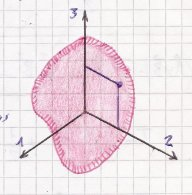
\includegraphics[scale=0.4]{images/fig_mc_rigid_body_inercia1.jpg}

El cambio de sistema se hace de acuerdo a
\[
	I_{ik}' = \sum_{\ell s} a_{i\ell} I_{\ell s} a_{ks}
\]
y en componentes,
\[
	\sum_q m_q ( \delta_{ik} {r'}^2_q - x'_i x'_k ) =  a_{i\ell} a_{ks} \sum_q m_q
	( \delta_{\ell s} r^2_q - x_\ell x_s )
\]
donde en el miembro izquierdo es $i \neq k$, y el derecho $\ell \neq s$
\[
	- \sum_q m_q x'_i x'_k =  - \sum_q m_q a_{i\ell} x_\ell a_{ks}  x_s 
\]
entonces 
\[
	I =
	\begin{pmatrix} \;
		I_{11} & I_{12} & I_{13} \\
		I_{21} & I_{22} & I_{23} \\ 
		I_{31} & I_{32} & I_{33} \\
	\end{pmatrix}
\]
siendo el triángulo superior valores repetidos. El tensor de inercia es simétrico por su 
definición. De los nueve componentes son independientes seis. Matemáticamente
\[
	I_{ik} = I_{ki}.
\]

Eligiendo convenientemente los ejes se puede llevar todo tensor simétrico a una forma
diagonal. En ese caso
% Todo tensor simétrico se puede llevar a una forma diagonal eligiendo bien los ejes del 
% sistema 123 fijo al cuerpo. Podemos conseguir una transformación $I \to I'$ tal que 
\[
	I' =
	\begin{pmatrix} \;
		I_{11}' & 0 & 0 \\
		0 & I_{22}' & 0 \\ 
		0 & 0 & I_{33}' \\
	\end{pmatrix}
\]
Los $I'_{ik}$ son los momentos principales de inercia (aquellos que están calculados sobre
{\it ejes principales de inercia}).

Cuando el cuerpo rígido tiene simetría pueden hallarse a ojo los ejes principales de inercia.
Como por ejemplo un cilindro:

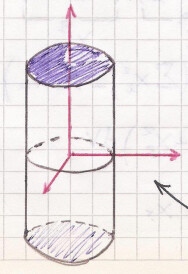
\includegraphics[scale=0.4]{images/fig_mc_rigid_body_ejesinercia0.jpg}

Sin embargo, los componentes del tensor dependen del tiempo debido a su movimiento,
\notamargen{Hay un tema acá con el tiempo $t$ y con la diagonalización.}

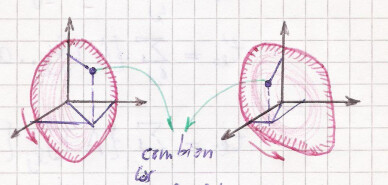
\includegraphics[scale=0.4]{images/fig_mc_rigid_body_ejesinercia1.jpg}

Entonces defino un sistema fijo al cuerpo. 
Para el cálculo de $I$ se usa un sistema fijo al cuerpo rígido. Si usamos un sistema inercial,
será $I_{ik}=I_{ik}(t)$ lo cual no es conveniente.

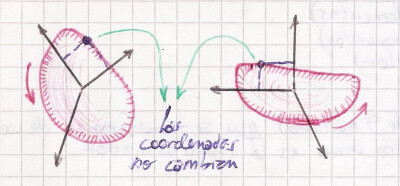
\includegraphics[scale=0.4]{images/fig_mc_rigid_body_ejesinercia2.jpg}

y ahora tengo $x\neq x(t)$ pero tengo cambiantes los ejes respecto al sistema inercial.
Tomaremos $123$ referido al sistema que rota y $XYZ$ referido al sistema que se traslada.
Necesitaré luego proyectar la rotación en el sistema inercial en los ejes que se trasladan
sobre el cuerpo.

Es conveniente elegir 123 con origen en el centro de masa y partícipes del movimiento del 
cuerpo rígido (clavados al mismo). Asimismo conviene elegir XYZ referidos al sistema inercial
coincidentes pero trasladados al centro de masa. Así los $I_{ik}$ resultan características
geométricas del cuerpo.

Finalmente, resulta 
\[
	T = \frac 1 2 M V_{cm}^2 + \frac 1 2 \left( I_{11} \Omega_1^2 + I_{22} \Omega_2^2 + I_{33} \Omega_3^2 \right)
\]
donde $I$ son los momentos principales de inercia \index{Inercia, momentos principales de}. Para obtener
esta expresión necesito elegir bien el sistema coordenado en el cuerpo rígido.

Los momentos principales de inercia están tabulados para diversos cuerpos geométricos.

\notamargen{Está un poco disconexo esto porque falta algo de esa clase. pág. 64}

Cumplen la siguiente propiedad,
\[
	I_i + I_j \geq I_k \quad \forall i,j,k
\]

% =================================================================================================
\section{El tensor de inercia}\index{Tensor de inercia}
% =================================================================================================

Siendo $I$ el tensor de inercia buscamos autovectores y autovalores del mismo. 
Es decir, soluciones a
\be
	I \vb{v} = \lambda \vb{v},
	\label{autovalores_inercia}
\ee
o bien en componentes
\be
	 \sum_{j=1}^3 I_{ij} v_j = \lambda v_i
\label{eigen_inercia}	 
\ee
que se trabaja así
\[
	 \sum_{j=1}^3 I_{ij} v_j - \lambda v_i =  \sum_{j=1}^3 ( I_{ij} - \delta_{ij}\lambda ) v_j = 0
\]
lo cual en extenso corresponde al siguiente sistema de tres ecuaciones
\[
	(I_{11} - \lambda)v_1 + I_{12} v_2 + I_{13} v_3 = 0
\]
\[
	I_{21} v_1 + (I_{22} - \lambda) v_2 + I_{23} v_3 = 0
\]
\[
	I_{31} v_1 + I_{32} v_2 + (I_{33} - \lambda) v_3 = 0
\]

Evidentemente, el determinante de la matriz $ I - \lambda \mathbb{1}$ tiene que ser nulo.
No obstante si $I$ fuese un tensor cualquiera no se puede garantizar tres raíces reales del polinomio
característico. Eso sucederá si la matriz del tensor resultara ser simétrica.

Ahora multiplicamos la ecuación \eqref{eigen_inercia} y su conjugada compleja (denotada por $^*$) por
$\sum_i v_i$ y $\sum_i v_i^*$, respectivamente, para obtener
\[
	\sum_i v_i \sum_{j=1}^3 I_{ij} v_j^* = \lambda^* \sum_i v_i^*  v_i
\]
\[
	\sum_i v_i^* \sum_{j=1}^3 I_{ij} v_j = \lambda \sum_i v_i v_i^*
\]

Ahora, restando ecuación a ecuación se tiene
\[
	\sum_i \sum_{j=1}^3 ( v_i I_{ij} v_j^* - v_i^* I_{ij} v_j ) =
	(\lambda^* - \lambda )\sum_i v_i^* v_i ,
\]
y como se puede cambiar de índices en el segundo sumando del miembro izquierdo, puesto que los índices están sumados y son
por ello mudos ({\it dummies}),
\[
	\sum_i \sum_{j=1}^3 ( v_i I_{ij} v_j^* - v_j^* I_{ji} v_i ) =
	(\lambda^* - \lambda )\sum_i v_i^* v_i 
\]
pero si usamos la propiedad de simetría del tensor de inercia $I_{ij}=I_{ji}$ entonces
\[
	0 = (\lambda^* - \lambda )\sum_i v_i^* v_i 
\]
de modo que como $\vb{v}$ es arbitrario se tiene la importante conclusión de que $\lambda^* = \lambda$.
Los autovalores del tensor de inercia son reales.

Se tienen $\lambda^s \in \mathbb{R}$ con $s=1,2,3$. Hay que asociar los autovectores, que pueden ser
complejos. Regresando al sistema de ecuaciones con un $\lambda^s$ puedo escribir todo en función
de cantidades $v_i/v_1$, esto es
% Si es por ejemplo $\lambda^s$ uno de los autovalores se pueden despejar
\be
	( v_1^s, v_2^s(v_1), v_3^s(v_1) )\: e^{i\phi}
	\label{autovector}
\ee
dado que una ecuación del sistema es linealmente dependiente [why?].

Como las cantidades $v_2/v_1, v_3/v_1 $ son reales es posible quedarse sin la fase del complejo (que es
la misma para todos) y hacer los componentes reales. 
Los autovectores darán información sobre {\it direcciones}, que necesitan ser reales [?].
La ec. \eqref{autovector} determina una dirección y es todo cuanto necesitaré. A partir de allí calcularé
el versor que me dará la dirección.
Se requerirá que la norma del vector sea unitaria, i.e. 
\[
	{v_1^s}^2 +  {v_2^s(v_1)}^2 + {v_3^s(v_1)}^2 = 1.
\]

Si en el sistema hay tres raíces idénticas, entonces la solución es $\mathbb{R}^3$, si hubiera dos es,
en cambio, un plano, $\mathbb{R}^2$.

Sean $\lambda^p \neq \lambda^s$ entonces 
\[
	\sum_i v_i^p \sum_{j=1}^3 I_{ij} v_j^s = \lambda^s \sum_i v_i^p  v_i^s
\]
\[
	\sum_i v_i^s \sum_{j=1}^3 I_{ij} v_j^p = \lambda^p \sum_i v_i^s v_i^p
\]
y restando ecuación a ecuación y cambiando subíndices como hiciéramos oportunamente,
\[
	\sum_i \sum_{j=1}^3 ( v_i^p I_{ij} v_j^s - v_i^s I_{ij} v_j^p ) =
	(\lambda^s - \lambda^p )\sum_i v_i^p v_i^s 
\]
luego como es nulo el miembro izquierdo resulta que 
\[
	\sum_i v_i^p v_i^s = 0
\]
de modo que $v^p$ y $v^s$ son ortogonales. Los autovectores correspondientes a autovalores 
diferentes son ortogonales.

Si hay autovalores iguales se puede completar a tres autovectores ortogonales con el método de
Gram-Schmidt [chequear si está bien escrito?].

En suma, con el tensor de inercia obtenemos tres direcciones ortogonales.
A partir de \eqref{autovalores_inercia}, multiplicando por delante por otro autovector $\vb{v}^{(p)}$,
\[
	\vb{v}^{(p) t} I \vb{v}^{(s)} = \lambda \vb{v}^{(p) t}  \vb{v}^{(s)},
\]
que define un producto matricial. En efecto, si se construye una matriz $V = ( v^s v^p v^q)$ la 
relación anterior será en todo su esplendor
\[
	V^t I V = \begin{pmatrix}
	           v_1^s & v_2^s & v_3^s \\
	           v_1^p & v_2^p & v_3^p \\
	           v_1^q & v_2^q & v_3^q
	          \end{pmatrix}
	          I
		\begin{pmatrix}
	           v_1^s & v_1^p & v_1^q  \\
	           v_2^s & v_2^p & v_2^q \\
	           v_3^s & v_3^p & v_3^q
	          \end{pmatrix}
\]

Como la norma de $\vb{v}$ es unitaria, se tiene además 
\[
	\vb{v}^t I \vb{v} = \lambda \vb{v}^t  \vb{v} = \lambda.
\]

Entonces
\[
	V^t I V = \lambda \mathbf{1}
\]
donde el $\mathbf{1}$ es la matriz identidad. 
De esta manera, $\lambda^s, \lambda^p, \lambda^q$ son los momentos principales de inercia
\[
	I = \begin{pmatrix}
	     \lambda^s & 0 & 0 \\
	     0 & \lambda^p & 0 \\
	     0 & 0  &  \lambda^q
	    \end{pmatrix}.
\]

Vale, además, que
\[
	\lambda^s = \sum_{ij}  v^s_i I_{ij} v^s_j > 0
\]
puesto que es una forma cuadrática y está definida positiva. 
\notamargen{En la carpeta dice que habría que demostrarlo}

Los autovectores en fila dan la matriz $A$ que se usará para pasar a un sistema {\it anclado} en el cuerpo rígido,
que será lo cual permitirá escribir la energía cinética $T$ como se ha visto.

\subsection{Simetrías y distribución de masa}

Un distribución de masa esférica $\rho(r)$ tiene todas las direcciones equivalentes,

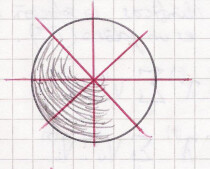
\includegraphics[width=0.2\textwidth]{images/fig_mc_inercia_simetrias_1.jpg}

Para la esfera maciza, en cualquier dirección tendremos eje principal de inercia: todos los momentos de
inercia serán iguales.
\[
	I = \lambda \begin{pmatrix}
	 1 & 0 & 0 \\
	 0 & 1 & 0 \\
	 0 & 0 & 1 
	\end{pmatrix}
\]

Para el paralelepípedo de la figura, rotando en $2\pi/3$ tengo la misma situación física (eje de simetría de orden tres), 
entonces tengo eje principal de inercia allí. Es un eje de simetría de orden tres.

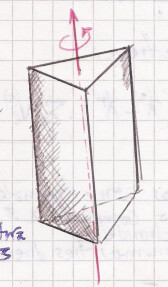
\includegraphics[width=0.2\textwidth]{images/fig_mc_inercia_simetrias_2.jpg}

En este caso $I = 1/2 U \vb{\Omega}^2 = 1/2 I ( \Omega_1^2 + \Omega_2^2 + \Omega_3^2 )$.

La caja se rota en $\pi/2$ en cada uno de los tres ejes y las direcciones no cambian. Eje de simetría de orden cuatro.
El cubo tiene los tres ejes de inercia iguales

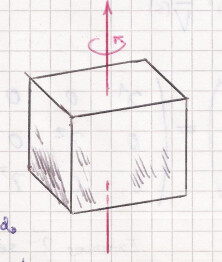
\includegraphics[width=0.2\textwidth]{images/fig_mc_inercia_simetrias_3.jpg}

Tetraedro no regular. Base equilátera. Un eje de rotación de algún orden es dirección de eje principal y en el
plano perpendicular a dicho eje están [?]

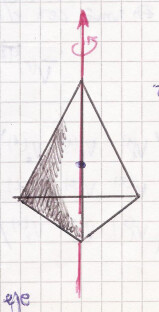
\includegraphics[width=0.2\textwidth]{images/fig_mc_inercia_simetrias_4.jpg}

La guitarra tiene simetría de imagen especular, como se visualiza en el lado derecho. En este caso tendremos
una dirección principal de inercia perpendicular al plano rojo y que pasa por el centro de masa del cuerpo.
Los otros dos ejes están contenidos en el plano.

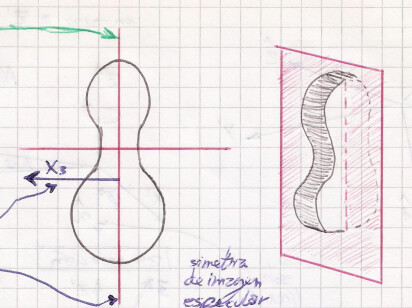
\includegraphics[width=0.2\textwidth]{images/fig_mc_inercia_simetrias_5.jpg}

[recorte o comentario de algún caso?]
Si $x_3$  es eje entonces $I_{13}, I_{23}$ se cancelan de a pares y anulan los productos de inercia.
\[
	\sum m^q x_2^q x_3^q 
\]
\[
	\begin{pmatrix}
	I_{11} & I_{12} & 0 \\
	I_{21} & I_{22} & 0 \\
	 0 & 0 & I_{33} 
	\end{pmatrix}
\]

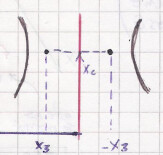
\includegraphics[width=0.2\textwidth]{images/fig_mc_inercia_simetrias_6.jpg}

La idea es que si pienso en planos siempre se hacen nulos los productos de inercia rotacionales [?].

Para la siguiente figura el plano de simetría es eje principal, luego es eje principal de inercia.
\begin{figure}[!htb]
	\begin{center}
	\includegraphics[width=0.15\textwidth]{images/fig_mc_ejesim.pdf}
	\end{center}
	\caption{}
\end{figure} 

\subsection{tensores -reubicar-}

Ante un cambio de coordenadas un vector transforma 
\[
	\vb{V}' = A \vb{V},
\]
donde $A$ es una matriz ortogonal. La idea es que no cualquier terna es un vector.
Un tensor tiene la propiedad de transformarse
\[
	t_{\ell s}' = \sum_i \sum_j a_{\ell i} a_{sj} t_{ij}
\]
o bien (haciendo énfasis en el producto matricial)
\[
	t_{\ell s}' = \sum_i \sum_j a_{\ell i} t_{ij} a_{sj}.
\]
Si recuperamos desde esta notación de sumatoria la estructura matricial notamos que 
\[
	t_{\ell s}' = \sum_i \sum_j [AT]_{\ell j} a_{sj}
\]
donde el factor $a_{sj}$ no se puede sumar así como está. Trasponiéndolo sí se puede,
y en efecto
\[
	t_{\ell s}' = \sum_i \sum_j [AT]_{\ell j} [A]_{js},
\]
de tal manera que la ley de transformación de un tensor de rango 2 es
\[
	T'= ATA^t.
\]

% =================================================================================================
\section{Ángulos de Euler}
% =================================================================================================

Ahora faltaría escribir todo en buenas coordenadas generalizadas. Lo habitual es escribir en función
de tres ángulos independientes. Euler inventó esta nomenclatura para estudiar el trompo.

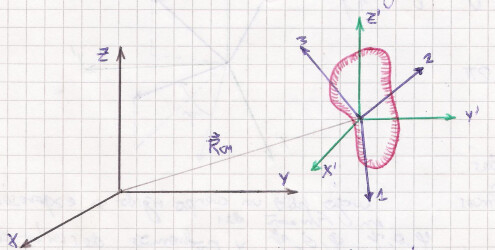
\includegraphics[width=0.5\textwidth]{images/fig_mc_sistema_euler_angles.jpg}

Los cosenos directores son nueve, pero son dependientes.
Consideraremos tres rotaciones, siendo su orden clave.

Se toma un sistema 123 inicialmente coincidente con uno XYZ paralelo al inercial, 123 tiene origen
en el centro de masa del cuerpo.

\begin{figure}[htb]
	\begin{center}
	\includegraphics[width=0.5\textwidth]{images/fig_mc_eulerangles.pdf}	 
	\end{center}
	\caption{}
\end{figure} 

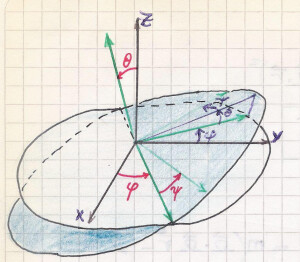
\includegraphics[width=0.5\textwidth]{images/fig_mc_sistema_euler_angles_carpeta.jpg}

La primera rotación define $\varphi$ 

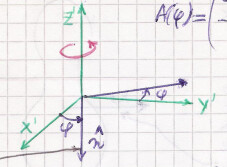
\includegraphics[width=0.5\textwidth]{images/fig_mc_euler_angles_1.jpg}

Se hace en torno a $z'$ a través de la matriz
\[
	A_1(\phi) = 
	\begin{pmatrix}
		\cos(\phi) & \sin(\phi) & 0 \\
		-\sin(\phi) & \cos(\phi) & 0 \\ 
		0 & 0 & 1  \\
	\end{pmatrix}
\]
El versor $\hat{n}$ está sobre la línea de nodos.

La segunda rotación define $\theta$ y es de acuerdo a la siguiente matriz

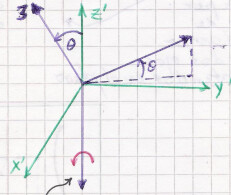
\includegraphics[width=0.5\textwidth]{images/fig_mc_euler_angles_2.jpg}

El eje inferior no se ha movido en esta rotación (obsérvese el 1 en la matriz)

\[
	A_2(\theta) = 
	\begin{pmatrix}
		1 & 0 & 0 \\
		0 & \cos(\theta) & \sin(\theta) \\ 
		0 & -\sin(\theta) & \cos(\theta)  \\
	\end{pmatrix}
\]

La tercr rotación define $\Psi$ y es en torno al eje $z$

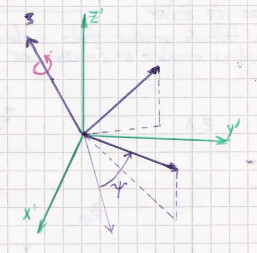
\includegraphics[width=0.5\textwidth]{images/fig_mc_euler_angles_3.jpg}

La matriz que la describe es
\[
	A_3(\psi) = 
	\begin{pmatrix}
		\cos(\psi) & \sin(\psi) & 0 \\
		-\sin(\psi) & \cos(\psi) & 0 \\ 
		0 & 0 & 1  \\
	\end{pmatrix}
\]

Luego, las coordenadas verifican
\[
	0 \leq \varphi,\Psi \leq 2\pi \qquad \qquad 0 \leq \theta \leq \pi
\]

Los ángulos $\theta,\varphi$ son variedades de los $\varphi,\theta$ de coordenadas esféricas.
Entonces, para un cuerpo rígido la velocidad de rotación se expresará en función de $\varphi,\theta,\psi$ y
sus derivadas $ \dot{\varphi},\dot{\theta},\dot{\psi} $ para describir también su evolución temporal.
En efecto,
\[
	\vb{\Omega} = \dot{\phi}\hat{z} + \dot{\theta}\hat{n} + \dot{\psi}\hat{3}
\]
y se debe expresar $\hat{z},\hat{n}$ en términos de $\hat{1},\hat{2}, \hat{3}$ (que son los ejes fijos en el cuerpo).
Como se tiene 
\[
	\hat{z} = \sin \theta \sin \psi \hat{1} + \sin \theta \cos \psi \hat{2} + \cos \theta \hat{3} \qquad 
	\hat{n} = \cos \psi \hat{1} - \sin \psi \hat{2}
\]
resulta la velocidad 
\[
	\vb{\Omega} = [\dot{\phi}\sin(\theta)\sin(\psi) + \dot{\theta}\cos(\psi) ]\hat{1} +
			[\dot{\phi}\sin(\theta)\cos(\psi) - \dot{\theta}\sin(\psi) ] \hat{2} +
			[\dot{\phi}\cos(\theta) + \dot{\psi} ]\hat{3}.
\]

Son estas componentes las que entran en la escritura del lagrangiano de un cuerpo libre como 
\[
	\Lag = T = \frac 1 2 M V_{cm}^2 + \frac 1 2 I_1 \Omega_1^2  + \frac 1 2 I_2 \Omega_2^2
	+ \frac 1 2 I_3 \Omega_3^2
\]

Ahora estamos interesados en el momento angular.
\[
	\vb{L}_0^{sist} = \vb{L}^{cm} + \vb{L}_{cm}^{sist} 
\]
\notamargen{Hay diferencia entre las expresiones del \vb{L} total. Resolver la convención!}
\[
	\vb{L} = \vb{L}_{orb} + \vb{L}_{spin} 
\]
\[
	\vb{L}_{spin} = \sum_i^N m_i ( \vb{x}_i' \times \vb{v}_i' )
\]
que están en el sistema $123$ (desde el centro de masa).
\[
	\vb{L}_{spin} = \sum_i^N m_i [ \vb{x}_i \times ( \vb{\Omega} \times \vb{x}_i ) ]
\]
\[
	\vb{L}_{spin} = \sum_i^N m_i \left[ \; 
	\vb{\Omega} (\vb{x}_i \cdot \vb{x}_i) - \vb{x}_i ( \vb{x}_i \cdot \vb{\Omega}) \; \right] 
\]
\[
	\vb{L}_{spin} = \sum_i^N m_i \left[ \; 
	\vb{\Omega} \sum_j^3 (x_j^{2i}) - \vb{r}_i \sum_\ell^3 x_\ell^i \Omega_\ell  \; \right] 
\]
\notamargen{Quilombo de notación!! ¡¡Fixear las diferentes $x$!!}
y la componente $k$-ésima será 
\[
	L_k = \sum_i^N m_i \left[ \; 
	\Omega_k \sum_j^3 (x_j^{2i}) - x_k^i \sum_\ell^3 x_\ell^i \Omega_\ell  \; \right] 
\]
\[
	L_k = \sum_i^N m_i \left[ \; 
	\sum_j^3 \delta_{kj} \Omega_j r_i^{2} - x_k^i \sum_\ell^3 x_\ell^i \Omega_\ell  \; \right] 
\]
\[
	L_k = \sum_j^3 \sum_i^N m_i \left[ \; 
	\delta_{kj} r_i^{2} - x_k^i x_j^i  \; \right] \Omega_j = \sum_j^3 I_{kj} \Omega_j 
\]
o vectorialmente
\[
	\vb{L}_{spin} = I \vb{\Omega}
\]
siendo $I$ el tensor de inercia. Es claro que $\vb{\Omega}$ y $\vb{L}$ no tienen porqué ser paralelos puesto que $I$ es
una matriz\footnote{En los problemas sencillos de física 1 era un escalar}. 
\notamargen{Se puede resolver en forma sencillla un cuerpo rígido a partir de $M d\vb{V}_{cm}/dt = \vb{F}$ y
considerando $I\vb{\omega}=\vb{\uptau}$, donde esto último es el momento angular de spin. Esto solamente para casos
sencillos, a lo F1.}
Explícitamente:
\[
	I_{kj} = \sum_i^N m_i \left[ \; \delta_{kj} \vb{x}_i^{2} - x_k^i x_j^i  \; \right]
\]
\[
	\begin{pmatrix}
		L_1 \\
		L_2 \\ 
		L_3  \\
	\end{pmatrix} 
	=
	\begin{pmatrix}
		I_{11} & I_{12} & I_{13} \\
		I_{21} & I_{22} & I_{23} \\ 
		I_{31} & I_{32} & I_{33}  \\
	\end{pmatrix}
	\begin{pmatrix}
		\Omega_1 \\
		\Omega_2 \\ 
		\Omega_3  \\
	\end{pmatrix} 
\]
\notamargen{$I=I(t)$ si lo describo desde un sistema inercial. $I \neq I(t)$ si lo describo desde un sistema no inercial.}

Si le tomamos la derivada temporal,
\[
	\dtot{\vb{L}}{t} = \dtot{}{t}\left( I \vb{\Omega} \right) = \vb{\uptau}
\]
donde resulta el torque con respecto al centro de masa. Si $I$ no depende del tiempo,
\[
	I \dtot{}{t}\left( \vb{\Omega} \right) = \vb{\uptau}
\]

El tensor depende del tiempo pués está derivado desde un sistema inercial, entonces 
\[
	\dtot{\vb{L}}{t} = \vb{\uptau},
\]
que para un observador rotante no vale [?] y debe escribirse 
\[
	\dtot{\vb{L}}{t}_{me} = \dtot{\vb{L}}{t}_{rot} + \vb{\Omega} \times \vb{L} = \vb{\uptau}
\]
donde \vb{\Omega} es la del sistema rotante.
Necesitaría un tensor escrito en el sistema cuerpo rígido (en los ejes principales). En este caso obtengo estas relaciones
triviales. En efecto,

Sean 1,2,3 los ejes principales, entonces $I$ es diagonal y
\[
	\vb{L}_{spin}
	=
	\begin{pmatrix}
		I_{11} & 0 & 0 \\
		0 & I_{22} & 0 \\ 
		0 & 0 & I_{33}  \\
	\end{pmatrix}
	\begin{pmatrix}
		\Omega_1 \\
		\Omega_2 \\ 
		\Omega_3  \\
	\end{pmatrix}
	=
	I \vb{\Omega}
\]

Luego se puede escribir el torque con el operador siguiente 
\[
	\left.\frac{d}{dt}\right|_{in} \Box = \left.\frac{d}{dt}\right|_{rot} \Box + \vb{\Omega} \times \Box 
	= \vb{\uptau}
\]
para cuando $\Box$ es el momento angular [?].
que es válida para sistemas rotantes (no aquellos que rotan y se trasladan).
En este caso \vb{\Omega} es la del sistema rotante (en un cuerpo rígido es la \vb{\Omega} del cuerpo rígido).

Se puede escribir también 
\[
	\left.\frac{d}{dt}\right|_{in} \vb{L}_{spin} = \vb{\Tau}_{cm}
\]
siendo la derivada de uns sitema XYZ, y \vb{\Tau} el torque del cuerpo rígido referido al centro de masa y
medido dese el sistema XYZ (inercial).
Entonces
\[
	\vb{\Tau}_{cm} = \left. \frac{d}{dt}\right|_{rot} \vb{L}_{spin} + \vb{\Omega} \times ( \vb{L}_{spin} )
\]
y
\[
	\vb{\Tau}_{cm} = \left. I \frac{d}{dt}\right|_{rot} \vb{\Omega} + \vb{\Omega} \times ( I \; \vb{\Omega} ).
\]
$I$ visto desde XYZ es $I=I(t)$ e $I$ desde 123 es constante.
\[
	\vb{\Tau}_{cm} =
	\begin{pmatrix} \;
		I_1 \dot{\vb{\Omega}}_1 \\
		I_2 \dot{\vb{\Omega}}_2 \\ 
		I_3 \dot{\vb{\Omega}}_3 \; \\
	\end{pmatrix}
	+
	\begin{vmatrix} \;
		\hat{1} & \hat{2} & \hat{3} \\
		\; \Omega_1 & \Omega_2 & \Omega_3 \\ 
		\; I_1\Omega_1 & I_2\Omega_2 & I_3\Omega_3 \; \\
	\end{vmatrix}	
\]

De este sistema resultan,
\begin{align*}
\Tau_1 = I_1 \dot{\Omega}_1 + (I_3-I_2) \: \Omega_2 \: \Omega_3 \\
\Tau_2 = I_2 \dot{\Omega}_2 + (I_1-I_3) \: \Omega_3 \: \Omega_1 \\
\Tau_3 = I_3 \dot{\Omega}_3 + (I_2-I_1) \: \Omega_1 \: \Omega_2
\end{align*}
que son las ecuaciones de Euler. 
Las mismas requieren $I$ en ejes principales, \vb{\Omega} en 1,2,3 (en función de $\phi,\theta,\psi$).
Es \vb{\Omega} la velocidad de rotación del sistema cuerpo rígido (rotante) respecto a un sistema XYZ
fijo en el centro de masa y coincidente con X'Y'Z' (inercial) a todo tiempo. Salvo la traslación del centro
de masa, este sistema XYZ será inercial.

Todo este tratamiento de ecuaciones de Euler es para el caso $\vb{L}_{spin} \equiv \vb{L}_{cm}^{sist}$, de
manera que no me importan las traslaciones del centro de masa.
\[
	\left.\frac{d}{dt}\right|_{XYZ} \vb{L}_{spin} = \vb{\Tau}_{cm} =
	\left.\frac{d}{dt}\right|_{123} \vb{L}_{spin} + \vb{\Omega} \times \vb{L}_{spin} 
\]

\notamargen{Hay que depurar bastante esta sección, y elegir una buena notación para el torque (no tengo un buen tau bold!)}
Para una peonza esférica son $I_1=I_2=I_3$.

% =================================================================================================
\subsection{La peonza simétrica}
% =================================================================================================

<<<<<<< .mine
Es lo que vulgarmente se conoce como {\it trompo}. Se eligen los ángulos de Euler.

\begin{figure}[!htb]
	\begin{center}
	\includegraphics[width=0.5\textwidth]{images/fig_mc_peonza1.pdf}	 
	\end{center}
	\caption{}
\end{figure} 

El cuerpo rígido se mueve con $\dot{\psi}$ pero no es necesario, en este ejemplo, que el sistema de coordenadas
lo haga puesto que hay una simetría. No se ven cambios para la rotación sobre el eje longitudinal.
||||||| .r505
Es lo que vulgarmente se conoce como {\it trompo}
=======
\notamargen{Junté comentarios de dos clases teóricas en esta sección.}
Es lo que vulgarmente se conoce como {\it trompo}.
La energía cinética se compone de una parte de traslación y una de rotación, es decir $T=T_{trasl} + T_{rot}$.
La velocidad angular del cuerpo y del sistema solidario al mismo es
>>>>>>> .r508
\[
	\vb{\Omega} = \dot{\varphi} \hat{z} + \dot{\theta} \hat{n} + \dot{\psi} \hat{x}_3
\]

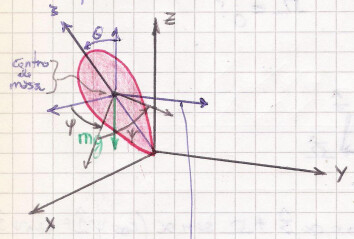
\includegraphics[width=0.5\textwidth]{images/fig_mc_peonza_segunda_1.jpg}

El sistema inercial se transporta al centro de masa, puesto que la idea es que se mide con respecto a un
sistema que sólo se traslada.
El sistema fijo al cuerpo garantiza un tensor independiente del tiempo, estacionaria \footnote{Es decir, una
distribución de masa que no depende del tiempo}. 

Cuando existe una simetría asociada no hace falta que las coordenadas sigan al cuerpo (aquellas que medirían
esa simetría). En este caso, si no proyecto sobre todas las coordenadas, ya no es la proyección de la 
velocidad.

La terna derecha que usamos para proyectar los ángulos de Euler tiene que estar en las direcciones de los
ejes principales de inercia, eso garantiza que podamos expresar la energía cinética de rotación según 
\[
	T_{rot} = \frac{1}{2} I_1 \Omega^2_ 1 + \frac{1}{2} I_2 \Omega^2_2 + \frac{1}{2} I_3 \Omega^2_3 
\]
<<<<<<< .mine
[todo es muy confuso aquí]
Velocidad angular del rígido $\dot{\psi} \neq 0$, coordenada $\psi=0$ pero $\psi=cte$ (no se entiende la trama).
Si tomo $\psi=0$ es $\hat{1}=\hat{n}$, la línea de nodos coincide con el eje $\hat{1}$.
En este caso la velocidad angular del cuerpo rígido proyctada en los ejes $123$ del mismo es
||||||| .r505
donde son 
=======
donde para el trompo son 
>>>>>>> .r508
\[
	\Omega_1 = \dot{\theta} \qquad \Omega_2 = \dot{\phi} \sin(\theta) \qquad \Omega_3 = \dot{\phi} \cos(\theta) + \dot{\psi}
\]
y debemos destacar que $\psi=0$ no es vínculo sino solo comodidad pues $\dot{\psi} \neq 0$ y es independiente.
<<<<<<< .mine
\notamargen{Si considero movimiento en $\psi$ trabajo mucho más la cuenta pero debería llegar a lo mismo.}

Este problema tiene tres grados de libertad porque el movimiento del centro de masa está vinculado
\[
	T_{trasl} = \frac 1 2 M \dot{\vb{R}}_{cm}^2
\]
\[
	\dot{\vb{R}}_{cm} = a \dot{\theta}_{cm} \hat{\theta}_{cm} + a \sin \theta \dot{\varphi_{cm}} \hat{\varphi}_{cm}
\]

Si no tiene simetría las velocidades angulares del sistema coordenado coinciden con las velocidades angulares del cuerpo rígido.
Si hay simetría, $\theta,\psi,\varphi$ podrán ser nulas con lo cual puede ser que no haga falta rotar el sistema rotante en 
todas las direcciones. En el ejemplo de la figura bajo estas líneas, $\theta$ y $\theta_{euler}$ concidenm y $\varphi$ y 
$\varphi_{euler}$ forman ángulo de $\pi/2$

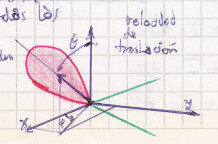
\includegraphics[width=0.5\textwidth]{images/fig_mc_rigid_body_peonza.jpg}

||||||| .r505
=======

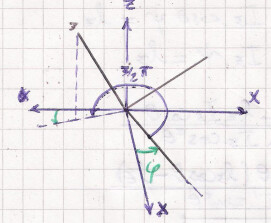
\includegraphics[width=0.35\textwidth]{images/fig_mc_peonza_segunda_2.jpg}

>>>>>>> .r508
Los vínculos pueden escribirse
\[
	\theta_e = \theta
\]
\[
	\phi_e + \frac{3}{2}\pi = \phi \; \longrightarrow \; \dot{\phi_e} = \dot{\phi}
\]
\[
	R^2_{cm} = a^2 = x_{cm}^2 + y_{cm}^2 + z_{cm}^2
\]
<<<<<<< .mine
donde $\theta, \phi$ y $r$ corresponden al centro de masas. 
Las coordenadas
||||||| .r505
\begin{figure}[htb]
	\begin{center}
	\includegraphics[width=0.5\textwidth]{images/fig_mc_peonza1.pdf}	 
	\end{center}
	\caption{}
\end{figure} 
y las coordenadas
=======

\begin{figure}[htb]
	\begin{center}
	\includegraphics[width=0.5\textwidth]{images/fig_mc_peonza1.pdf}	 
	\end{center}
	\caption{}
\end{figure} 
y las coordenadas
>>>>>>> .r508
\begin{align*}
	x &= a \sin(\theta) \cos\left( \frac{\pi}{2}-\phi_e \right) = a \sin(\theta) \sin( \phi_e ) \\
	y &= a \sin(\theta) \sin\left( \frac{\pi}{2}-\phi_e \right) = -a \sin(\theta) \cos( \phi_e ) \\
	z &= a \cos(\theta)
\end{align*}
<<<<<<< .mine
y la velocidad de traslación
||||||| .r505
y la velocidad
=======

Luego, la energía $T_{trasl}$ se puede poner en términos de los ángulos de Euler, a través de la velocidad del 
centro de masas, que verifica 
>>>>>>> .r508
\[
	V_{cm}^2 = \dot{x}^2 + \dot{y}^2 + \dot{z}^2 = a^2 \dot{\theta}^2 + a^2 \sin(\theta)^2 \dot{\phi}^2.
\]
<<<<<<< .mine
La energía cinética es suma de la de traslación y la de rotación,
||||||| .r505
y el lagrangiano finalmente
=======

Pero esta velocidad del centro de masas tiene parte de la cinética de rotación, y entonces se puede reescribir
la energía cinética como 
>>>>>>> .r508
\[
	T = \frac{1}{2} M (a^2 \dot{\theta}^2 + a^2 \sin(\theta)^2 \dot{\phi}^2) + \frac{1}{2} I_1 \dot{\theta}^2
	+ \frac{1}{2} I_2 \sin(\theta)^2 \dot{\phi}^2) + \frac{1}{2} I_3 (\dot{\phi} \cos(\theta) + \dot{\psi})^2 
\]
pero por la simetría $I_1=I_2\equiv I$ de modo que 
\[
<<<<<<< .mine
	G = \frac{1}{2} M a^2 (\dot{\theta}^2 + \sin(\theta)^2 \dot{\phi}^2) + \frac{1}{2} I ( \dot{\theta}^2 +
	\sin(\theta)^2 \dot{\phi}^2 ) + \frac{1}{2} I_3 (\dot{\phi} \cos(\theta) + \dot{\psi})^2, 
||||||| .r505
	\Lag = \frac{1}{2} M a^2 (\dot{\theta}^2 + \sin(\theta)^2 \dot{\phi}^2) + \frac{1}{2} I ( \dot{\theta}^2 +
	\sin(\theta)^2 \dot{\phi}^2 ) + \frac{1}{2} I_3 (\dot{\phi} \cos(\theta) + \dot{\psi})^2 
=======
	T = \frac{1}{2} M a^2 (\dot{\theta}^2 + \sin(\theta)^2 \dot{\phi}^2) + \frac{1}{2} I ( \dot{\theta}^2 +
	\sin(\theta)^2 \dot{\phi}^2 ) + \frac{1}{2} I_3 (\dot{\phi} \cos(\theta) + \dot{\psi})^2, 
>>>>>>> .r508
\]
<<<<<<< .mine
y el lagrangiano será
||||||| .r505
=======

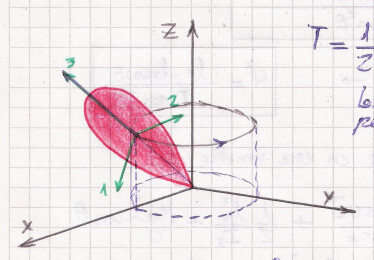
\includegraphics[width=0.35\textwidth]{images/fig_mc_peonza_segunda_3.jpg}

y el lagrangiano es, finalmente,
>>>>>>> .r508
\[
	\Lag = \frac{1}{2} ( M a^2 + I ) (\dot{\theta}^2 + \sin(\theta)^2 \dot{\phi}^2) +  
		\frac{1}{2} I_3 (\dot{\phi} \cos(\theta) + \dot{\psi})^2  - m g a \cos(\theta)
\]
donde los primeros dos términos representan una rotación pura si tomo 
\[
	( M a^2 + I ) \equiv I' 
\]
donde $I'$ es otro momento de inercia.
\begin{figure}[htb]
	\begin{center}
	\includegraphics[width=0.5\textwidth]{images/fig_mc_peonza2.pdf}	 
	\end{center}
	\caption{}
\end{figure} 

<<<<<<< .mine
Debido a la ciclicidad en el lagrangiano se conservan 
\[
	p_\theta = I' \sin^2 \theta \dot{ \varphi } + I_3 ( \dot{\psi} + \dot{\varphi} \cos\theta ) \cos \theta 
\]
\[
	p_\varphi = l_z 
\]
\[
	p_\psi = I_3 ( \dot{\psi} + \dot{ \varphi }\cos \theta )
\]
pero esta última es en realidad $l_3$ porque el cuerpo rígido presenta una invariancia al moverse en torno a los ejes $\hat{3}$
y $\hat{z}$.

||||||| .r505
=======
Este sistema tiene como constantes de movimiento
\be
	p_\varphi = \dpar{\Lag}{\dot{\varphi}} = I' \sin^2 \theta \dot{ \varphi } +
	I_3 (  \dot{\psi} + \dot{\varphi} \cos \theta ) \cos \theta
	\label{lz}
\ee
\be
	p_\psi = \dpar{\Lag}{\dot{\psi}} = I_3 (  \dot{\psi} + \dot{\varphi} \cos \theta )
	\label{l3}
\ee

La variación de $\varphi,\psi$ son ambas rotaciones rígidas, entonces si se conservan sus momentos
canónicos conjugados será $p_\varphi \equiv$ proyección de \vb{L} sobre el eje $z$ ($\ell_z$) y
$p_\psi \equiv$ proyección de \vb{L} sobre el eje $3$ ($\ell_3$).

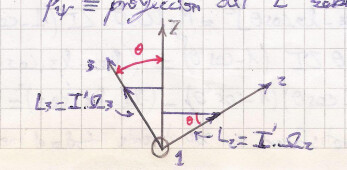
\includegraphics[width=0.35\textwidth]{images/fig_mc_peonza_segunda_4.jpg}

En la figura sobre estas líneas se ve que $\ell_z$ es lo que corresponde.
\[
	I_3 \Omega_3 \cos \theta = I_3 ( \dot{\psi} + \dot{\varphi} \cos \theta )\sin \theta
\]
\[
	I \Omega_2 \sin \theta = I' \sin^2 \theta \dot{ \varphi }
\]
y $\ell_z$ es una constante que está presente siempre porque las proyecciones no dependen de $\varphi$.

Además, se conserva la energía (y coincidirá con el hamiltoniano); es más engorroso resolver las
ecuaciones de Euler-Lagrange.
Usaremos las constantes $\ell_z,\ell_3$ (según los momentos conjugados en \eqref{lz} y \eqref{l3}).
Entonces podemos despejar
\[
	\dot{\psi} = \frac{\ell_3}{I_3} + \frac{(\ell_3 \cos\theta - \ell_z)\cos\theta}{I'\sin^2\theta}
\]
y
\[
	\dot{\varphi} = \frac{\ell_z - \ell_3 \cos \theta}{I'\sin^2\theta}
\]

Amasando y haciendo álgebra se llega a un problema en una única variable $\theta$,
\[
	E = \frac 1 2 I' \dot{\theta}^2 + \frac{(\ell_z - \ell_3 \cos \theta)^2}{2I'\sin^2\theta} +
	\frac{1}{2}\frac{\ell_3^2}{I_3} + M g a \cos\theta
\]
y redefino
\[
	E' \equiv E - \frac{1}{2} \frac{\ell_3^2}{I_3} = 
	\frac 1 2 I' \dot{\theta}^2 + \frac{(\ell_z - \ell_3 \cos \theta)^2}{2I'\sin^2\theta} + M g a \cos\theta
\]
donde el {\it potencial} resultante tendrá alguna forma como se muestra en la figura debajo, para $0 \leq \theta \leq \pi$

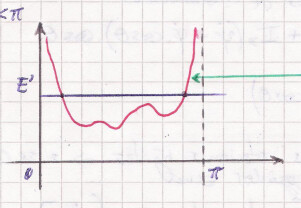
\includegraphics[width=0.35\textwidth]{images/fig_mc_peonza_segunda_5.jpg}

Los puntos $E'=V$ son un polinomio cúbico en $\cos\theta$. 
Haciendo un poco de álgebra en la energía $E'$,
\[
	2I'(E'- Mga\cos\theta)(1-\cos^2\theta) - (\ell_z - \ell_3 \cos \theta)^2 =
	I'^2 \dot{\theta}^2 \sin^2\theta = I'^2 \left( \dtot{\cos\theta}{t} \right)^2. 
\]
Este polinomio debe satisfacer ser no nulo durante todo el movimiento. Luego, definiendo
$q\equiv \cos\theta$, se tiene que como cambia de signo en el límite $q\to +\infty$ y en $q\to -\infty$
debe tener una raíz. Además $q=1$ y $q=-1$ están debajo del cero.
Entonces tendrá una raíz en $q>1$

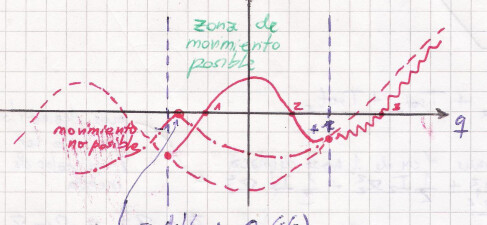
\includegraphics[width=0.5\textwidth]{images/fig_mc_peonza_segunda_6.jpg}

Tiene una raíz doble en $q<1$ (ver figura sobre estas líneas) y entonces $\theta_0 (cte)$ equivale a una
órbita circular de fuerzas centrales. $\dot{\theta}=0$

El trompo se mueve entre $\theta_m$ y $\theta_M$ y además tiene tres movimientos dados por los ángulos
\[
	\begin{cases}
	\varphi \quad \text{ ángulo de precesión }\\
	\theta \quad \text{ ángulo de nutación } \\
	\psi \quad \text{ ángulo de rotación propia } 
	\end{cases}
\]

El eje del trompo se puede representar en una esfera (ver figura bajo estas líneas).
La imagen superior de la derecha corresponde al caso en que $\dot{\varphi}$ cambia de signo.
La imagen inferior se da si es largado desde condiciones iniciales $\dot{\varphi}=0$ y 
$\dot{\theta}=0$ (desde la raíz?)

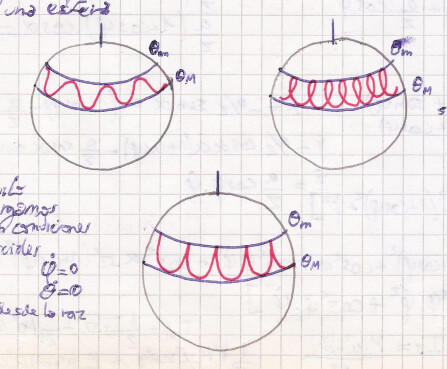
\includegraphics[width=0.5\textwidth]{images/fig_mc_peonza_segunda_7.jpg}

>>>>>>> .r508
Luego hay unos interesantes comentarios sobre la ubicación de los ejes. El famoso ``bajo ejes''.
\[
	T = T_{trasl} + T_{rot} + T_{acopl}
\]
y el último es nulo si elegimos el origen común O=O'= centro de masa.
\[
	\vb{V} = \vb{V}_{cm} + \Omega \times \vb{r}
\]
También es $T_{acopl}=0$ si $V_0=0$ (aquí también se anula $T_{trasl}$).

\notamargen{Comentario respecto a Euler angles: las rotaciones que dan los ángulos de Euler son
sobre ejes distintos; esto da el problema, no son una base ortogonal $z,\xi,\hat{3}$}

% ~~~~~~~~~~~~~~~~~~~~~~~~~~~~~~~~~~~~~~~~~~~~~~~~~~~~~~~~~~~~~
\begin{ejemplo}{\bf Problema 4c}

Suponemos que en esta situación hay rodadura.

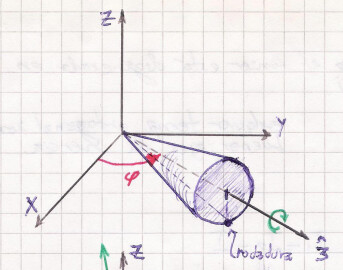
\includegraphics[width=0.5\textwidth]{images/fig_mc_cono_rodando_1.jpg}

La condición de rodadura proporciona bastante información.

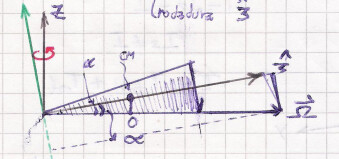
\includegraphics[width=0.5\textwidth]{images/fig_mc_cono_rodando_2.jpg}

Queremos escribir el vector velocidad angular en función de los ejes definidos en la figura.
Entonces
\[
	\vb{\Omega} = \Omega \cos \alpha \hat{3} + \Omega \sin \alpha ( \cos \psi \hat{1} + \sin \psi \hat{2} )
\]
Luego, como
\[
	\vb{v}_0 = 0 = \vb{v}_{cm} + \vb{\Omega} \times \vb{x}_0,
\]
será
\[
	v_{cm} = \Omega a \sin \alpha
\]
y el centro de masa describe una circunferencia en torno a $z$, de radio $a \cos \alpha$ con velocidad tangencial
dada por 
\[
	v_{cm} = \dot{\varphi} a \cos \alpha.
\]

Ahora se puede calcular la energía cinética, que será 
\[
	T = \frac 1 2 v_{cm}^2 + \frac 1 2 \Omega^t I \Omega 
\]
\[
	T = \frac 1 2 m a^2 \cos^2 \alpha \dot{\varphi}^2 + \frac{1}{2}( I_1\Omega_1^2 + I_2\Omega_2^2 + I_3\Omega_3^2)
\]
y usando que $I_1=I_2$ por simetría
\[
	T = \frac 1 2 \cos^2 \alpha ( ma^2 + I_1 + I_3 \mbox{cotg}^2 \alpha ) \dot{\varphi}^2
\]
\notamargen{Habría que hacer la cuenta prolija y llegar bien al resultado final.}

\includegraphics[width=0.5\textwidth]{images/fig_mc_cono_rodando_3.jpg}
 
\end{ejemplo}


% =================================================================================================
\section{Teorema de Steiner}
% =================================================================================================

\[
	\vb{x} = \vb{U} - \vb{a}  
\]
\[
	I_{ij}^0 = \sum_s^N m^s ( \delta_{ij} x_s^2 - x_i^s x_j^s )
\]
\[
	I_{ij}^0 = \sum_s^N m^s ( \delta_{ij} ( \vb{U}_s - \vb{a} )^2 - (U^s_i - a_i) ( U^s_j - a_j ) )
\]
\begin{figure}[htb]
	\begin{center}
	\includegraphics[width=0.5\textwidth]{images/fig_mc_steiner1.pdf}	 
	\end{center}
	\caption{}
\end{figure} 
Trasladamos el punto (con el sistema de ejes paralelo al del centro de masa) sin rotarlo. Eso es importante.
\[
	I_{ij}^0 = \sum_s^N m^s \left[  \delta_{ij} ( U_s^2 + a^2 - 2Ua ) -
			( U^s_iU^s_j + a_i a_j - a_i U^s_j - a_j U^s_i ) \right]
\]
\[
	I_{ij}^0 = \sum_s^N m^s ( \delta_{ij} U_s^2 - U^s_iU^s_j ) + \sum_s^N m^s ( \delta_{ij} a^2 - a_i a_j )
			- \sum_s^N m^s \delta_{ij} 2 U^s a  + \sum_s^N m^s ( a_i U^s_j + a_j U^s_i )
\]
pero las dos últimas sumatorias son nulas, y
\[
	I_{ij}^0 = \sum_s^N m^s ( \delta_{ij} U_s^2 - U^s_iU^s_j ) + \sum_s^N m^s ( \delta_{ij} a^2 - a_i a_j )
		= I_{ij}^{cm}  + M ( \delta_{ij} a^2 - a_i a_j )
\]

Esto sale de
\[
	\sum_s^N m^s \delta_{ij} U^s a = \delta_{ij} a \sum_s^N m^s  U^s  = 0
\]
puesto que es nula la suma en $s$. Porque 
\[
	0 = \sum_s^N m^s \vb{U}^s = \sum_s^N m^s ( U_1^s \hat{1} + U_2^s \hat{2} + U_3^s \hat{3} )
\]
pero como es vectorial vale para cada coordenada 
\[
	0 = \sum_s^N m^s U_i^s \qquad \forall i=1,2,3
\]
\[
	0 = \sum_s^N m^s U_i^s a
\]
\begin{figure}
	\begin{center}
	\includegraphics[width=0.5\textwidth]{images/fig_mc_steiner2.pdf}	 
	\end{center}
	\caption{}
\end{figure} 
La moraleja es que trasladar en un solo eje conserva la diagonalidad del tensor de inercia.

% =================================================================================================
\section{Sistemas no inerciales}
% =================================================================================================

\notamargen{Habría que pasar los \vb{r} a \vb{x}.} 

\begin{figure}
	\begin{center}
	\includegraphics[width=0.7\textwidth]{images/fig_sist_rotantes.pdf}	 
	\end{center}
	\caption{Sistemas rotantes.}
\end{figure} 

\vb{\Omega} es la velocidad angular del sistema no inercial. $\ddot{\vb{R}}$ es la aceleración del 
sistema no inercial. Ambas se miden sólo desde el sistema inercial.

\[
	\vb{r} = \vb{R} + \vb{r}'
\]
\[
	\left.\dtot{\vb{r}}{t}\right|_{in} =
			\left.\dtot{\vb{R}}{t}\right|_{in} + \left.\dtot{\vb{r}'}{t}\right|_{in}
\]
si despejamos la derivada respecto del sistema primado,
\[
	\left.\dtot{\vb{r}'}{t}\right|_{in} = \left.\dtot{\vb{r}}{t}\right|_{in} 
				- \left.\dtot{\vb{R}}{t}\right|_{in}
\]
y usamos 
\[
	\left.\dtot{\vb{r}'}{t}\right|_{in} = \left.\dtot{\vb{r}'}{t}\right|_{no in} +
				\vb{\Omega} \times \vb{r}'
\]
va resultando 
\[
	\left. \frac{d}{dt}\left( {\left.\dtot{\vb{r}'}{t}\right|_{no in}} \right) \right|_{in}  =  
			\left.\dtot[2]{\vb{r}}{t}\right|_{in}  - \left.\dtot[2]{\vb{R}}{t}\right|_{in} 
			- \left. \dtot{(\vb{\Omega} \times \vb{r}')}{t}\right|_{in}
\]
\[
	\left.\dtot[2]{\vb{r}'}{t}\right|_{no in}  + \vb{\Omega} \times \left.\dtot{\vb{r}'}{t}\right|_{no in}
		 = \vb{a}|_{in} - \ddot{\vb{R}}|_{in} - \left. \dtot{\vb{\Omega}}{t}\right|_{in} \times \vb{r}' 
				+ \vb{\Omega} \times \left. \dtot{ \vb{r}'}{t}\right|_{in}
\]
donde hemos usado que 
\[
	\left. \dtot{\vb{\Omega}}{t} \right|_{in} = \left. \dtot{\vb{\Omega}}{t} \right|_{no in} \qquad \qquad
	\left. \dtot{\vb{R}}{t} \right|_{in} = - \left. \dtot{\vb{R}}{t} \right|_{no in}
\]
\[
	\left.\dtot[2]{\vb{r}'}{t}\right|_{no in}  + \left( \vb{\Omega} \times \left.\dtot{\vb{r}'}{t}\right|_{no in} \right)
		 = \vb{a}|_{in} - \ddot{\vb{R}}|_{in} 
		 - \left[\left. \dtot{\vb{\Omega}}{t}\right|_{no in} + \vb{\Omega} \times \vb{\Omega} \right] \times \vb{r}' 
		+ \vb{\Omega} \times \left[ \left. \dtot{ \vb{r}'}{t}\right|_{no in} + \vb{\Omega} \times \vb{r}' \right]
\]
\[
	\left. \vb{a}'\right|_{no in}   = \vb{a}|_{in} - \ddot{\vb{R}}|_{in} 
		 - \dot{\vb{\Omega}} \times \vb{r}'  -  \vb{\Omega} \times \left.\dot{\vb{r}}' \right|_{no in} 
		- \vb{\Omega} \times \left( \vb{\Omega} \times \dot{\vb{r}}' \right) 
		- \vb{\Omega} \times  \left. \dtot{ \vb{r}'}{t}\right|_{no in} 
\]
\[
	\left. \vb{a}'\right|_{no in}  = \ddot{\vb{r}}  - \ddot{\vb{R}}
		 - \dot{\vb{\Omega}} \times \vb{r}'  -  2 \vb{\Omega} \times \left.\dot{\vb{r}}' \right|_{no in} 
		- \vb{\Omega} \times \left( \vb{\Omega} \times \dot{\vb{r}}' \right)
\]

Vale la pena aclarar la deduccion,
\[
	\left. \dtot{\vb{r}}{t} \right|_{in} = \left. \dtot{\vb{R}}{t} \right|_{in} + \left. \dtot{\vb{r}'}{t} \right|_{no in}
	+ \vb{\Omega} \times \vb{r}' 
\]
pero si es $\vb{R}=0$ se tiene $\vb{r}=\vb{r}'$ y entonces
\[
	\left. \dtot{\vb{r}}{t} \right|_{in} =  \left. \dtot{\vb{r}'}{t} \right|_{no in} + \vb{\Omega} \times \vb{r}' 
\]
donde el sistema no inercial es el rotante.

\begin{ejemplo}{\bf Sistema rotante con resorte divertido}

El sistema físico está mostrado en la ilustración bajo estas líneas.

\includegraphics[width=0.4\textwidth]{images/fig_mc_rotantes_ejemplo_bloque1.jpg}

El siguiente esquema permite ver la descomposición de fuerzas

\includegraphics[width=0.4\textwidth]{images/fig_mc_rotantes_ejemplo_bloque2.jpg}

\[
	Y_A(t) = Y_B(t) = Y_0 \sin (\Omega t) \hat{y} \qquad \vb{\omega} = \omega \hat{z}
\]
siendo $\omega$ una constante.
\[
	F_y' = - k y' \hat{y}' \qquad F_z' = k(z_0' - z) \hat{z}'
\]
y la aceleración es 
\[
	m \vb{a}' = - ky' \hat{y}' + k (z_0' - z) \hat{z}' + y_0 \Omega^2 \sin (\Omega t) \hat{y}
	- 2 m \omega \hat{z}' \times ( \omega \hat{z}' \times [ y' \hat{y}' + z' \hat{z}' ] ) 
	- 2 m \omega \hat{z}' \times ( \dot{y}' \hat{y}' + \dot{z}' \hat{z}' )
\]
 
\includegraphics[width=0.4\textwidth]{images/fig_mc_rotantes_ejemplo_bloque3.jpg}

\[
	\hat{y} = (\hat{y}\cdot\hat{x}')\hat{x}' +  (\hat{y}\cdot\hat{x}')\hat{y}' + 
	\underbrace{(\hat{y}\cdot\hat{z}') }_{=0}\hat{z}'
	= \sin(\omega t) \hat{x}' + \cos(\omega t) \hat{y}'
\]
y como $\delta = \pi/2 - \omega t$ se tiene 
\[
	\cos \delta = \cos ( \pi/2 - \omega t ) = \sin ( \omega t )
\]

Luego,
\[
	\hat{y}' ) \quad m \ddot{y}' = -k y' + 2 m \omega^2 y' + m y_0 \Omega^2 \sin(\Omega t)\cos(\omega t)
\]
\[
	\hat{z}' ) \quad m \ddot{z}' = k ( z_0' - z' )
\]
\[
	\hat{x}' ) \quad 0 = F_v + 2m\omega \dot{y}' + m y_0 \Omega^2 \sin(\Omega t)\sin(\omega t)
\]
donde la última componente no me interesa.
De las componentes $\hat{y}',\hat{z}'$ surge la solución (que es del tipo oscilador armónico)
\[
	\ddot{z}' + \frac k m z' = \frac k m z_0'
\]
de manera que 
\[
	z(t) = A_z \cos\left( \sqrt{\frac{k}{m}} t + \varphi_z \right) + z_0'.
\]

\[
	\ddot{y}' + \left( \frac k m - 2\omega^2 \right) y' =  m y_0 \Omega^2 \sin( \Omega t) \cos (\omega t)
\]
donde se ve que es un oscilador forzado.
Si el sistema está forzado, entonces no se conserva la energía.

Pero además puede verse por el hecho de que el lagrangiano depende del tiempo a través de los vínculos. Es decir que
tenemos vínculos dependientes del tiempo.
\[
	\sin( \Omega t) \cos (\omega t) = \frac{1}{2} \sin( [\Omega + \omega] t ) +  \frac{1}{2} \sin( [\Omega - \omega] t )
\]
Propongo una solución particular 
\[
	y_{part} = A_+ \cos( [\Omega + \omega] t ) + B_+ \sin( [\Omega + \omega] t ) 
		+ A_- \cos([\Omega - \omega] t) + B_- \sin([\Omega - \omega] t)
\]

Luego de hacer el álgebra correspondiente se llega a los valores de las amplitudes que son 
\[
	A_+ = \frac{ y_0 \Omega^2 }{ 2[ ( k/m - 2 \omega^2 ) - (\Omega + \omega)^2 ] } \;
	A_- = \frac{ y_0 \Omega^2 }{ 2[ ( k/m - 2 \omega^2 ) - (\Omega - \omega)^2 ] } \; B_+=0 \; B_-=0
\]

Puede haber resonancia si el denominador se hace muy chico. Juntando todo,
\[
	y'(t) = y_h'(t) + y'_{part}(t)
\]
\begin{multline*}
	y'(t) = A_{\parallel} \cos\left( \sqrt{ \frac k m - 2 \omega^2 } + \varphi_H \right) + \\
	\frac{ y_0 \Omega^2 }{ 2[ ( k/m - 2 \omega^2 ) - (\Omega + \omega)^2 ] } \cos([\Omega +\omega] t ) + 
	\frac{ y_0 \Omega^2 }{ 2[ ( k/m - 2 \omega^2 ) - (\Omega - \omega)^2 ] } \cos([ \Omega - \omega ] t )
\end{multline*}
\end{ejemplo}

\begin{ejemplo}{\bf Problema 7 --retitular luego--}

\includegraphics[width=0.4\textwidth]{images/fig_mc_rotantes_prob7_1.jpg}

Consideramos un cuerpo libre,
\[
	\dot{\vb{\omega}} = 0 \qquad \vb{A} = \vb{R} = \vb{\omega} \times ( \vb{\omega} \times \vb{R} )
\]
\[
	\vb{F}  = -\frac{GMm}{\rho^3}\vb{\rho}
\]

Entonces la aceleración es
\[
	\vb{a}'= \underbrace{ -\frac{GMm}{\rho^3}\vb{\rho} - \vb{\omega} \times ( \vb{\omega} \times \vb{R}) }_{\text{Esto da } 
	\vb{g} } - 2 \vb{\omega} \times \dot{\vb{x}}'- \vb{\omega} \times ( \vb{\omega} \times \vb{x}') 
\]

\includegraphics[width=0.4\textwidth]{images/fig_mc_rotantes_prob7_2.jpg}

Y las fuerzas
\[
	\vb{F} = \vb{T} + m \vb{g}
\]
\[
	\vb{T} = ( \vb{T}\cdot\vb{x}') \vb{x}' + ( \vb{T}\cdot\vb{y}') \vb{y}' + ( \vb{T}\cdot\vb{z}') \vb{z}' =
	-\frac{Tx}{\ell} \hat{x}' +  -\frac{Ty}{\ell} \hat{y}' + \frac{T}{\ell}(\ell-z) \hat{z}'
\]
\[
	m \vb{a}  = \vb{T} + m \vb{g} - 2 m ( \vb{\omega} \times  \dot{\vb{x}}') -
	m ( \vb{\omega} \times [ \vb{\omega} \times \vb{x}'] )
\]
Si se tiene $|\vb{\omega}| \ll \Omega $, se puede despreciar $\omega$ (se tiran los términos cruzados) y entonces se simplifica a
\[
	\hat{x}' ) \quad m \ddot{x}' = - \frac{T}{\ell} x' + 2 m \omega \dot{y}' \cos \lambda
\]
\[
	\hat{y}' ) \quad m \ddot{y}' = - \frac{T}{\ell} y' - 
	2 m \omega \left( \dot{x}' \cos \lambda + \dot{z} \sin \lambda \right)
\]
\[
	\hat{z}' ) \quad m \ddot{z}' = \frac{T(\ell -z)}{\ell} - m g + 2 m \omega \dot{y}' \sin \lambda
\]

Ahora aproximo con pequeñas oscilaciones y tengo $z$ aproximadamente constante, luego $\dot{z} = \ddot{z} = 0$ de
tal manera que se puede despejar del sistema anterior 
\[
	T = m g - 2 m \omega \dot{y} \sin \lambda
\]
e incorporándola en las otras dos, se tiene 
\[
	\ddot{x}' = - \frac{g}{\ell} x' + 2 \omega \dot{y}' \cos \lambda
\]
\[
	\ddot{y}' = - \frac{g}{\ell} y' - 2 \omega \dot{x}' \cos \lambda 
\]

Definiendo $g/\ell \equiv K^2$ y $\alpha \equiv \omega \cos \lambda $ las dos anteriores lucen como 
\[
	\ddot{x}' = - K^2 \dot{x} + 2 \alpha \dot{y}' \qquad \ddot{y}' = - K^2 \dot{y} - 2 \alpha \dot{x}',
\]
es decir que se tiene un sistema acoplado. Para desacoplarlo se puede utilizar números complejos de la forma siguiente,
definiendo una variable compleja
\[
	X = x' + i y'
\]
De esta forma 
\[
	\ddot{X} = \ddot{x}' + i \ddot{y}' = - K^2 (x' + i y') - 2 i \alpha (x' + i y'),
\]
\[
	\ddot{X} = - K^2 X - 2 i \alpha \dot{X}
\]
donde entonces el vínculo con la solución del problema es 
\[
	x'(t) = \mathfrak{Re}(x) \qquad y'(t) = \mathfrak{Im}(x)
\]

Resolviendo para condiciones inicales
\[
	x_0' = 0, \quad \dot{x}_0' = 0 \qquad \qquad y_0' = A, \quad \dot{y}_0' = 0
\]
se tienen
\[
	x'(t) = A \cos ( \sqrt{g/\ell} t ) \sin( \omega \cos \lambda t )
\]
\[
	y'(t) = A \cos ( \sqrt{g/\ell} t ) \cos( \omega \cos \lambda t )
\]
Se puede ver entonces que no se conserva el plano de oscilación del péndulo sino que va rotando.
\end{ejemplo}


% =================================================================================================
\section{Lagrangiano de un sistema no inercial que se traslada}
% =================================================================================================

\notamargen{En la carpeta están desarrollados separadamente}

El lagrangiano de una partícula libre en un sistema inercial es
\[
	\Lag_0 = \frac 1 2 m v_0^2 - U,
\]
que lleva por extremar la acción a las correspondientes ecuaciones de movimiento.
Note que utilizamos $U$ para el potencial para evitar confusiones con $V$ que será la velocidad entre sistemas.
Supongamos ahora otro sistema $K'$ como se ve en la figura,

\includegraphics[width=0.4\textwidth]{images/fig_mc_no_inercial_ejemplo_1.jpg}

que se traslada. Por eso sus orígenes están separados por un vector $X(t)$ que depende del tiempo.

Se tiene, evidentemente,
\[
	\vb{x}_0 = \vb{x}(t) + \vb{X}(t) \qquad \vb{v}_0 = \vb{v}'(t) + \vb{V}(t)
\]

Entonces escribiendo $\Lag'$, donde hay que insistir en que esto no significa que se escribe el
lagrangiano desde el sistema $K'$ sino que el lagrangiano se expresa en función de las coordenadas
y momentos en $K'$, se tiene 
\[
	\Lag' = \frac{1}{2} m v^2 - U(\vb{x})
\]
\[
	\Lag' = \frac{1}{2} m ( v' + V )^2 - U(\vb{x})
\]
\[
	\Lag' = \frac{1}{2} m {v'}^2 + m \: \vb{V}\cdot\vb{v}' + \frac{1}{2} m V^2 - U(\vb{x}) 
\]

El término en $V^2$ se puede despreciar puesto que equivale a un término $df/dt$ que cumpliría
\[
	\dtot{f}{t} = \frac{1}{2} m V^2 \qquad \qquad f = \frac{1}{6} m V^3 + K
\]
y además 
\[
	 m \vb{V}\cdot\vb{v}' =  m \: \vb{V} \cdot\dtot{\vb{x}'}{t\phantom{'}} = 
	 \frac{d}{dt}\left( m \: \vb{V} \cdot \vb{x}' \right) - m \dtot{ \vb{V} }{t} \vb{x}' 
\]
que corresponde al procedimiento conocido en la práctica como {\it hacer partes}.
El primer término es una derivada total y por ello se tira porque equivale a una derivada total con 
respecto al tiempo. Entonces,
\[
	\Lag' = \frac{1}{2} m {v'}^2 - m \dtot{\vb{V}}{t}\cdot\vb{x}' - U(\vb{x}).
\]

Las ecuaciones de Euler-Lagrange serán 
\notamargen{Explicar esa notación con vectores dividiendo; es una notación, capo.}
\[
	\dtot{}{t} \left( \dpar{\Lag'}{\vb{v}'} \right) - \dpar{\Lag'}{\vb{x}'} =
		m \dot{ \vb{V} } + m \dtot{\vb{v}'}{t} + \dtot{U}{\vb{x}'} = 0,
\]
o bien
\[
	m \vb{a}' = -\dtot{U}{\vb{x}'} - m \vb{A}
\]
donde en el lado derecho el primer término es $m\vb{a}$ (la aceleración del sistema inercial) y el segundo una fuerza
ficticia $m\vb{A}$ que surge de medir en términos de un sistema que está acelerado con respecto a uno inercial.
\notamargen{Acá hay que revisar bien la convención de inercial y no inercial!}
Expresamos $v=v(V,v')$ con lo cual aparecen en el $\Lag'$ las fuerzas ficticias y expreso $T$ en 
función de coordenadas que se hallan sobre un sistema no inercial.

\includegraphics[width=0.4\textwidth]{images/fig_mc_no_inercial_ejemplo_2.jpg}

En el caso de la parte de rotación, los vectores $\vb{x}=(x,y,z)$ y $\vb{x}'=(x',y',z')$ son los mismos como vector pero
están descritos en diferentes sistemas de coordenadas.

Se tiene 
\[
	\left. \dtot{\vb{x}}{t} \right|_{in} = \left. \dtot{\vb{x}}{t} \right|_{rot} + \vb{\Omega} \times \vb{x}
\]
donde el subíndice $in$ refiere al sistema fijo mientras que $rot$ refiere, como se espera, al sistema que rota.
Esta ecuación es
\[
	\vb{v} = \vb{v}' + \vb{\Omega} \times \vb{x}'
\]
y el lagrangiano 
\[
	\Lag = \frac 1 2 m ( \vb{v} + \vb{\Omega} \times \vb{x} )^2 - U - m \: \vb{x} \cdot \vb{A},
\]
que descompone a 
\[
	\Lag = \frac 1 2 m \: v^2 + m \: \vb{v} \cdot ( \vb{\Omega} \times \vb{x} ) - U 
	- m \: \vb{x} \cdot \vb{A} + \frac 1 2 (\vb{\Omega} \times \vb{x} )^2,
\]
el lagrangiano válido en cualquier sistema.

El cálculo de las ecuaciones de Euler-Lagrange da 
\[
	\dtot{}{t}\left( \dpar{\Lag}{\vb{v}} \right) = m \dtot{\vb{v}}{t} + m \dot{\vb{\Omega}} \times \vb{x} + m \vb{\Omega} \times \vb{v}
\]
\[
	\dpar{\Lag}{\vb{x}} = \dtot{}{\vb{x}} \left( m \vb{v} \cdot ( \vb{\Omega} \times \vb{x} ) \right) - 
	\Nabla U - m \vb{A} + \frac 1 2 \dtot{}{t} ( \vb{\Omega} \times \vb{x} )^2
\]
y utilizando la ec. del apéndice ([escalar de un vector y un producto vectorial])
\[
	\dtot{}{\vb{x}} \left( m \vb{v} \cdot ( \vb{\Omega} \times \vb{x} ) \right) = m \vb{v} \times \vb{\Omega},
\]
y usando el producto escalar de dos productos vectoriales (apéndice vectores) y el vectorial de un vector y un producto vectorial,
\[
	( \vb{\Omega} \times \vb{x} )^2 = \Omega^2 x^2 - ( \vb{\Omega} \cdot \vb{x} )^2
\]
\[
	\frac 1  2 m \dtot{}{\vb{x}}( \Omega^2 x^2 - ( \vb{\Omega} \cdot \vb{x} )^2 ) = 
	m ( (\vb{\Omega} \cdot \vb{\Omega} ) \vb{x} - ( \vb{\Omega} \cdot \vb{x} ) \vb{\Omega} ) =
	m \vb{\Omega} \times ( \vb{x} \times \vb{\Omega} ).
\]

Entonces,
\[
	m \: \dtot{\vb{v}}{t} = m \vb{x} \times \dot{\vb{\Omega}} + 2 m \vb{V} \times \vb{\Omega} - m \vb{\Omega} \times ( \vb{\Omega} \times \vb{x} )
	- \Nabla U - m \vb{A}
\]
y se ha recuperado la expresión de aceleración en el sistema no inercial.

Esto de aquí abajo estaba en la versión pretérita. Habría que confraternizarlo con lo anterior.
\[
	\left. \dtot[2]{\vb{r}}{t} \right|_{in} = 
	\left. \frac{d}{dt}\left( \left. \dtot{\vb{r}}{t} \right|_{rot} + \vb{\Omega} \times \vb{r} \right) \right|_{rot}
	+ \vb{\Omega} \times \left( \left. \dtot{\vb{r}}{t} \right|_{rot} + \vb{\Omega} \times \vb{r} \right)
\]
\[
	\left. \dtot[2]{\vb{r}}{t} \right|_{in} = 
	\left. \dtot[2]{\vb{r}}{t} \right|_{rot}  \; +  \; \left.\dtot{\vb{\Omega}}{t}\right|_{rot} \times \vb{r}
	 \;  + \; 2 \vb{\Omega} \times \left. \dtot{\vb{r}}{t} \right|_{rot} 
	 \;  + \;  \vb{\Omega} \times \left( \vb{\Omega} \times \vb{r} \right)
\]

% =================================================================================================
\section{Sistemas rotantes}
% =================================================================================================

Considero dos sistemas, XYZ inercial y X'Y'Z' rotante (no inercial).

\[
	\vb{U}' = A \vb{U} 
\]
donde $A$ es la matriz del cambio de coordenadas (una transformación ortogonal) y $U$ es una descripción
desde el XYZ y $U'$ una descripción desde el X'Y'Z'.

Haremos unas derivadas utilizando la regla de la cadena,
\[
	\dtot{U}{t} = \dtot{U_x}{t}\hat{x} + \dtot{U_y}{t}\hat{y} + \dtot{U_z}{t}\hat{z} 
\]
donde es $U = U(x,y,z)$, pero ahora si es $U = U(x',y',z')$ se tiene en cambio
\[
	\dtot{U}{t} = \dtot{U_x'}{t}\hat{x}' + U_x' \dtot{\hat{x}'}{t} + 
	\dtot{U_y}{t}\hat{y} + U_y' \dtot{\hat{y}'}{t} + \dtot{U_z}{t}\hat{z} + U_z' \dtot{\hat{z}'}{t}
\]

Pero X'Y'Z' es un sistema ortogonal y sus versores cumplen condiciones de ortogonalidad entonces
\[
	\hat{x}'\cdot\hat{x}' = \hat{y}'\cdot\hat{y}' = \hat{z}'\cdot\hat{z}' = 1
\]
\[
	\hat{x}'\cdot\hat{y}' = \hat{x}'\cdot\hat{z}' = \hat{y}'\cdot\hat{z}' = 0
\]

Ahora tenemos que hacer las variaciones de las dos ecuaciones precedentes. De la primera
\be
	 \hat{x}'\cdot\delta\hat{x}' = \hat{y}'\cdot\delta\hat{y}' = \hat{z}'\cdot\delta\hat{z}' = 0
\label{variac1}	 
\ee
y de la segunda
\be
	\hat{x}'\cdot\delta\hat{y}' + \hat{y}'\cdot\delta\hat{x}' = 0 \qquad \qquad 
	\hat{x}'\cdot\delta\hat{z}' + \hat{z}'\cdot\delta\hat{x}' = 0 \qquad \qquad 
	\hat{y}'\cdot\delta\hat{z}' + \hat{z}'\cdot\delta\hat{y}' = 0 \qquad \qquad 
\label{variac2}	
\ee

Asimismo, una variación $\delta\hat{x}'$ arbitraria puede escribirse como
\[
	\delta\hat{x}' = \delta \alpha_{xx}\hat{x}' + \delta \alpha_{xy}\hat{y}' + \delta \alpha_{xz}\hat{z}' 
\]
donde es $\delta \alpha_{xx}=0$ debido al primer miembro de \eqref{variac1}. Notemos que $\delta \alpha_{xy}$ significa
una variación en $\hat{x}'$ proyectada en $\hat{y}'$. Del mismo modo escribimos
\[
	\delta\hat{y}' = \delta \alpha_{yx}\hat{x}' + \delta \alpha_{yz}\hat{z}' 
\]
\[
	\delta\hat{z}' = \delta \alpha_{zx}\hat{x}' + \delta \alpha_{zy}\hat{y}' 
\]
donde ya hemos anulado las que sabemos son nulas por el mismo argumento. Usando \eqref{variac2} se tiene también
\[
	\hat{x}'\cdot\delta\hat{z}' =  - \hat{z}'\cdot\delta\hat{x}' \qquad 
	\hat{x}'\cdot\delta\hat{y}' =  - \hat{y}'\cdot\delta\hat{x}'
\]
que pasan respectivamente a
\[
	\hat{x}'\cdot\delta\alpha_{zx} =  - \hat{z}'\cdot\delta\alpha_{xz} \qquad 
	\hat{x}'\cdot\delta\alpha_{yx} =  - \hat{y}'\cdot\delta\alpha_{xy}
\]

Pero las variaciones son tres (¿?)
\[
	\delta\vb{\alpha} = ( \delta\alpha_x, \delta\alpha_y, \delta\alpha_z).
\]

La delta de un versor tiene componentes en los otros tres versores (no en el mismo versor)
\[
	\delta\hat{x}' = \delta \alpha_{xy}\hat{y}' + \delta \alpha_{xz}\hat{z}'
\]
\[
	\delta\hat{y}' = \delta \alpha_{yx}\hat{x}' + \delta \alpha_{yz}\hat{z}'
\]
\[
	\delta\hat{z}' = \delta \alpha_{zx}\hat{x}' + \delta \alpha_{zy}\hat{y}'
\]
pero proyectando
\[
	\hat{x}'\cdot\delta\hat{z}' =  - \hat{z}'\cdot\delta\hat{x}' \qquad \longrightarrow \qquad 
					\delta\alpha_{zx} = -\delta\alpha_{xz}
\]
\[
	\hat{y}'\cdot\delta\hat{z}' =  - \hat{z}'\cdot\delta\hat{y}' \qquad \longrightarrow  \qquad 
					\delta\alpha_{zy} = -\delta\alpha_{yz}
\]
\[
	\hat{x}'\cdot\delta\hat{y}' =  - \hat{y}'\cdot\delta\hat{x}' \qquad \longrightarrow  \qquad 
					\delta\alpha_{yx} = -\delta\alpha_{xy}
\]

Con las siguientes definiciones 
\[
	\delta\alpha_{zx} \equiv \delta\alpha_y \qquad 
	\delta\alpha_{yz} \equiv \delta\alpha_x \qquad
	\delta\alpha_{xy} \equiv \delta\alpha_z 
\]
estamos autorizados a escribir
\[
	\delta\hat{x}' = \delta \alpha_z \hat{y}' - \delta \alpha_y \hat{z}'
\]
\[
	\delta\hat{y}' = - \delta \alpha_z \hat{x}' + \delta \alpha_x \hat{z}'
\]
\[
	\delta\hat{z}' = \delta \alpha_y \hat{x}' - \delta \alpha_x \hat{y}'
\]
\begin{figure}[htb]
	\begin{center}
	\includegraphics[width=0.4\textwidth]{images/fig_mc_rotaciones.pdf}	 
	\end{center}
	\caption{}
\end{figure} 
La rotación infinitesimal puede verse como un vector 
\[
	\delta\vb{\alpha} = \delta\alpha_x \hat{x} + \delta\alpha_y \hat{y} +  \delta\alpha_z \hat{z} 
\]
\[
	\frac{\delta\vb{\alpha}}{\delta t} = \Omega_x \hat{x} + \Omega_y \hat{y} +  \Omega_z \hat{z} 
\]
donde hemos hecho $\Omega_i = \delta\alpha_i/\delta t$, es decir que identificamos las componentes del vector velocidad angular. 
En términos de las nuevas variables
\[
	\frac{ \delta \hat{x}' }{ \delta t } = \Omega_z \hat{y}' - \Omega_y \hat{z}'
\]
\[
	\frac{ \delta \hat{y}' }{ \delta t }  = - \Omega_z \hat{x}' + \Omega_x \hat{z}'
\]
\[
	\frac{ \delta \hat{z}' }{ \delta t } = \Omega_y \hat{x}' - \Omega_x \hat{y}'
\]

Entonces, juntando todo 
\[
	\dtot{\vb{U} }{t} = \dtot{U_x'}{t} \hat{x}' + \dtot{U_y}{t}\hat{y} + \dtot{U_z}{t}\hat{z} + 
	U_x' ( \Omega_z \hat{y}' - \Omega_y \hat{z}' ) + U_y'( - \Omega_z \hat{x}' + \Omega_x \hat{z}' ) 
	+ U_z'( \Omega_y \hat{x}' - \Omega_x \hat{y}' ),
\]
y acomodando según los versores tenemos 
\[
	\dtot{\vb{U} }{t} = \left[ \dtot{U_x'}{t} - U_y' \Omega_z + U_z' \Omega_y  \right] \hat{x}' + 
	\left[ \dtot{U_y}{t} + U_x' ( \Omega_z - U_z' \Omega_x \right] \hat{y}  + 
	\left[ \dtot{U_z}{t} + U_y' \Omega_x - U_x' \Omega_y \right] \hat{z} 
\]
\notamargen{Me gustaba la identificación $\left.\frac{d}{dt} \right|_{X'Y'Z'}$ el primer gran término en la derivada
total del vector $\vb{U}$.}
Los términos asociados a la velocidad angular {\it entran} como un producto vectorial de manera que podemos 
colapsar la notación en 
\[
	\left.\frac{d}{dt}\right|_{in} \vb{U} = \left.\frac{d}{dt} \right|_{rot} \vb{U} + \vb{\Omega} \times \vb{U}.
\]

Recordemos que 
\[
	\vb{\Omega} \times \vb{U}' = \begin{vmatrix}
	                              \hat{x}' & \hat{y}' & \hat{z}' \\
	                              \Omega_x & \Omega_y  & \Omega_z \\
	                              U_x' & U_y' & U_z' 
	                             \end{vmatrix}.
\]

Pero $\vb{\Omega}$ es un vector que puede variar en el tiempo. El eje de rotación puede variar en el tiempo,

\includegraphics[scale=0.4]{images/fig_mc_rotaciones_porqueria.jpg}

Suponiendo que \vb{U} solo rota 

\includegraphics[scale=0.4]{images/fig_mc_rotaciones_u_solorota.jpg}

\[
	\frac{\delta \alpha}{\delta t} U \sin \beta = \Omega U \sin \beta = \vb{\Omega} \times \vb{U}
\]

Un observador rotante vería $dU/dt|_{rot} = 0$ porque no cambian las componentes. Él sería partícipe del movimiento de \vb{U} y 
como la velocidad de rotación de \vb{U} es \vb{\Omega} entonces \vb{U} se ve quieta.

\begin{ejemplo}{\bf Rotación en $\hat{z}$}

Consideremos una rotación en torno a $\hat{z}'$ de manera que como $\delta\hat{z}'=0$ entonces  
$\delta\alpha_x=\delta\alpha_y=0$

Luego, se tienen 
\[
	\delta\hat{x}' = \delta\alpha_z \hat{y}' \qquad \delta\hat{y}' = - \delta\alpha_z \hat{x}'
\]
y entonces debe ser
\[
	\delta \alpha_z \equiv \omega_z . 
\]
\begin{figure}[htb]
	\begin{center}
	\includegraphics[width=0.4\textwidth]{images/fig_mc_rotzej.pdf}	 
	\end{center}
	\caption{}
\end{figure} 

\includegraphics[scale=0.4]{images/fig_mc_rotaciones_ej_rotz.jpg}

\notamargen{¿Este gráfico y el anterior son lo mismo?}
\end{ejemplo}


\subsection{Lagrangiano en un sistema rotante}

Dado el lagrangiano usual de partícula sometida a potencial $V$,
\[
	\Lag = \frac{1}{2} m v^2 - V(\vb{x}),
\]
queremos ver qué forma adopta en un sistema rotante como el de ejes primados 

\includegraphics[scale=0.4]{images/fig_mc_rotaciones_ejes_primados.jpg}

La velocidad verifica 
\[
	\vb{v} = \vb{v}' + \Omega \times \vb{x}
\]
donde $ \vb{x} = \vb{x}'$ puesto que los orígenes de ambos sistemas coinciden.
Entonces,
\[
	\Lag = \frac{1}{2} m ( \vb{x}' + \vb{\Omega} \times \vb{x} )^2 - V(\vb{r})
\]
donde luego de hacer el álgebra del cuadrado resulta 
\[
	\Lag = \frac{1}{2} m \vb{v}'^2 + m \vb{v}' \cdot ( \vb{\Omega} \times \vb{x} ) + 
		\frac{1}{2} m ( \vb{\Omega} \times \vb{x} )^2 - V(\vb{x})
\]
donde los últimos tres términos puede agruparse en un potencial efectivo $ U = U(\vb{x}, \vb{v})$
tal que 
\[
	U = - m \vb{v}' \cdot ( \vb{\Omega} \times \vb{x} ) - 
		\frac{1}{2} m ( \vb{\Omega} \times \vb{x} )^2 + V(\vb{x}).
\]
Entonces 
\[
	\Lag = \frac{1}{2} m \vb{v}'^2 - U(\vb{x},\vb{v}).
\]

Esto es el lagrangiano que escribiría un observador del sistema rotante.
Allí se puede pensar que aparece un potencial $U$ dependiente de la velocidad que es fuente de todas
las fuerzas, ficticias y reales.
\[
	V_{coriolis} = - m \vb{v}' \cdot ( \vb{\Omega} \times \vb{x} )  
\]
\[
	V_{centrifugo} = \frac{1}{2} m ( \vb{\Omega} \times \vb{x} )^2 + V(\vb{x})
\]

La fuerza, puesto que es un potencial que depende de la velocidad, se obtiene a partir de  
\[
	\vb{F} = -\dpar{U}{q_i} + \frac{d}{dt} \left( \dpar{U}{\dot{q}_i} \right).
\]

Si la velocidad de rotación es baja, $\Omega \sim 0 $ a primer orden el lagrangiano de una partícula
libre en un sistema rotante es 
\[
	\Lag \approx \frac{1}{2} m \vb{v}'^2 - m \vb{v}' \cdot ( \vb{\Omega} \times \vb{x} ) ,
\]
puesto que el potencial centrífugo es cuadrático en la velocidad angular.
Para una partícula libre sometida a un campo electromagnético es
\[
	\Lag = \frac{1}{2} m \vb{v}'^2 - \frac{q}{2c} \vb{v} \cdot ( \vb{B} \times \vb{x} )
\]

Esto es el teorema de Larmor y 
\[
	\vb{\omega} = \frac{q}{2 m c} \vb{B}
\]
es la llamada frecuencia de Larmor.

Podemos definir un operador 
\notamargen{El cuadrado argumento del operador debiera ser un ente en negrita -vectorial-.}
\[
	\left.\dtot{}{t}\right|_{inercial} \vb{\Box} =  \left.\dtot{}{t}\right|_{rotante} \vb{\Box}
	+ \vb{\omega } \times \vb{ \Box },
\]
y entonces
\[
	\vb{F} = m \dtot[2]{x}{t} = m \left( \dtot{}{t} + \vb{\Omega} \times 
	\left[ \left.\dtot{x}{t}\right|_{rot} + \vb{\Omega} \times \vb{x} \right] \right)
\]
\[
	m \vb{a}_{cm} = - 2 m ( \vb{v}\times\vb{\Omega}) - m \vb{\Omega} \times (\vb{\Omega}\times\vb{x}) + \vb{F}
\]
con $d\vb{\Omega}/dt = 0$




% =================================================================================================
\section{Movimiento de un cuerpo asimétrico}
% =================================================================================================

\[
	\vb{L}_{spin} = I \vb{\Omega}
\]
y como la energía se conserva es
\[
	E = T + V
\]
\[
	E = T_{trasl} + T_{rot} + V(R_{cm})
\]
donde cada una se conserva separadamente.

\begin{figure}[htb]
	\begin{center}
	\includegraphics[width=0.4\textwidth]{images/fig_mc_asimbod.pdf}	 
	\end{center}
	\caption{}
\end{figure} 

Usaremos una notación en la cual el subíndice refiere a referido a y el supraíndice a de qué puntos/puntos
\[
	\left.\vb{L}\right|_{0}^{sist} = \left.\vb{L}_{orb}\right|_{0}^{cm} + \left.\vb{L}_{spin}\right|_{cm}^{sist}  
\]
\[
	\left.\frac{d\vb{L}^{orb}}{dt}\right|_{in} = \vb{\tau}_0^{cm} = \vb{R}_{cm} \times \vb{F} =
							\vb{R}_{cm} \times - M g \hat{z} \neq 0
\]
de tal manera que el $\vb{L}^{orb} \equiv \vb{L}_0^{cm}$ no se conserva.

El que se conserva es $\vb{L}^{spin}$ pues pensamos la $\vb{F}=M\vb{g}$ aplicada en el centro de masa que es el origen
y que tiene $\vb{R}_{cm}=0$.
\[
	\vb{L}^{spin} = L_1 \hat{1} + L_2 \hat{2} + L_3 \hat{3} = I_1\Omega_1 \hat{1} + I_2\Omega_2 \hat{2} + I_3\Omega_3 \hat{3}
\]
y podemos escribir
\[
	T_{rot} = \frac{1}{2} \left( I_1\Omega_1^2 + I_2\Omega_2^2 + I_3\Omega_3^2 \right)
\]
\[
	T_{rot} = \frac{L_1^2}{2 I_1} + \frac{L_2^2}{2 I_2} + \frac{L_3^2}{2 I_3}
\]
\[
	1  = \frac{L_1^2}{2 I_1 T_{rot}} + \frac{L_2^2}{2 I_2 T_{rot}} + \frac{L_3^2}{2 I_3 T_{rot}}
\]
\begin{figure}[htb]
	\begin{center}
	\includegraphics[width=0.4\textwidth]{images/fig_mc_asimbod2.pdf}	 
	\end{center}
	\caption{}
\end{figure} 
Entonces, si se da que $I_3 > I_2 > I_1$ se tiene 
\[
	L_{spin}^2 = L_1^2 + L_2^2 + L_3^2 \qquad L^2 =  I_1^2\Omega_1^2 + I_2^2\Omega_2^2 + I_3^2\Omega_3^2
\]
donde como se conservan $T_{rot} \equiv T$ y $L_{spin} \equiv L$ 
\[
	2 T = \frac{L_1^2}{I_1} + \frac{L_2^2}{I_2} + \frac{L_3^2}{I_3} \qquad L^2 = L_1^2 + L_2^2 + L_3^2
\]
de la primera deducimos un elipsoide de semiejes en $L_i$ y de la segunda una esfera de radio $L$ en $L_i$.
\notamargen{Esto está super oscuro. No sé qué se quiso decir, tal vez se halle explicado mejor en la carpeta.}
\begin{figure}[htb]
	\begin{center}
	\includegraphics[width=0.4\textwidth]{images/fig_mc_asimbod3.pdf}	 
	\end{center}
	\caption{}
\end{figure} 
\[
	2 I_3 T > 2 I_2 T > 2 I_1 T
\]
\[
	L^2 > 2 I_3 T	\qquad L_1^2 + L_2^2 + L_3^2 > \frac{I_3}{I_1} L_1^2 + \frac{I_3}{I_2} L_2^2  + L_3^2
\]
\[
	L_1^2 \left( \frac{I_1 - I_3}{I_1} \right) + L_2^2 \left( \frac{I_2 - I_3}{I_1} \right)  > 0
\]
pero esto no vale. Asimismo tampoco vale que 
\[
	L^2 < 2 I_1 T
\]
y resulta 
\[
	2 I_3 T > L^2 > 2 I_1 T
\]
entonces $L_{spin}$ (su punta) se mueve en la intersección de una esfera y un elipsoide.
Estos movimientos son periódicos.

La peonza tiene movimientos estables para la rotación en torno a $\hat{x}_1, \hat{x}_3$ pero inestables en
torno a $\hat{x}_2$. El movimiento puede resolverse mediante ecuaciones de Euler.
Es estable rotar en torno al mayor o menor momento de inercia lo que generará un movimiento oscilatorio
para \vb{\Omega} ($\omega^2 > 0$), en cambio es inestable rotar en torno al momento de inercia intermedio, lo cual generará
un movimiento armónico para \vb{\Omega} ($\omega^2 < 0$).

Con \vb{L} constante si \vb{L }$\parallel$ \vb{\Omega} entonces ambos son constantes (corresponde a una rotación). Se consigue 
con \vb{\Omega} en la dirección del eje principal. Si \vb{L }$\nparallel$ \vb{\Omega} entonces \vb{\Omega} oscila en torno a
\vb{L}.



% \bibliographystyle{CBFT-apa-good}	% (uses file "apa-good.bst")
% \bibliography{CBFT.Referencias} % La base de datos bibliográfica

\end{document}
